\chapter{Vorbereitungs-Testphase der Anwendungen}\label{sec:pre-study}

Dieser Abschnitt beschreibt eine vorbereitende Testphase, die den im folgenden Kapitel \ref{sec:study} dargestellten Versuchsdurchführung vorgelagert ist. Ziel dieser Phase war es, erste gebrauchstauglichkeitsbezogene Probleme der entwickelten Anwendung zu identifizieren. Auf diese Weise sollen potenzielle Schwächen frühzeitig erkannt werden, um vor Beginn der eigentlichen Testreihen entsprechende Anpassungen vorzunehmen oder relevante Aspekte gezielt in die Versuchsdurchführung zu integrieren.

\section{Methodik}
In diesem Kapitel wird die methodische Herangehensweise der vorbereitenden Testphase dargestellt, mit dem Fokus auf die Identifikation erster gebrauchstauglichkeitsbezogener Schwächen sowohl der Anwendungen, des infrastrukturellen Aufbaus und der Rätsel. Ziel war es, die technische Infrastruktur bereitzustellen und durch erste Testspielsitzungen einen Eindruck von der Schwierigkeit der Rätsel sowie der Bedienbarkeit der Anwendung zu gewinnen. Hierzu wurde ein qualitatives Erhebungsverfahren angewandt.

\subsection{Forschungsdesign}

Um erste gebrauchstauglichkeitsbezogene Schwächen der Anwendung identifizieren zu können, wurde das praxisorientierte Thinking-Aloud-Verfahren eingesetzt. Der Fokus lag dabei insbesondere auf der Evaluation der implementierten Steuerungselemente der Player- und Watcher-Anwendungen, sowie der Rätsel.

\subsection{Erhebnungsinstrumente}

Zur Erfassung der im Rahmen der Thinking-Aloud-Methode geäußerten Gedanken und Hinweise der Probanden, wurde ein Beobachtungsprotokoll als Erhebungsinstrument eingesetzt. Die verbalen Äußerungen wurden stichpunktartig dokumentiert, wobei der Fokus auf spontanen Kommentaren zur Steuerung, zu den Rätseln sowie zu aufgetretenen Schwierigkeiten lag. Auf eine audiovisuelle Aufzeichnung wurde bewusst verzichtet, um die Testsituation möglichst natürlich zu gestalten. Die protokollierten Aussagen wurden anschließend einer qualitativen Inhaltsanalyse unterzogen.

\subsection{Stichporengröße}\label{sec:pre-study-sample}

Bei der Festlegung der Stichprobengröße musste der Aspekt des \say{Verbrauchens von Probanden} berücksichtigt werden, da die ausgewählten Teilnehmer nicht an der späteren Hauptuntersuchung teilnehmen durften. Aufgrund ihrer Vorerfahrung mit dem Anwendungsszenario bestünde die Gefahr einer Voreingenommenheit, wodurch die Ergebnisse der späteren Wirkungsanalyse verfälscht werden könnten. Aus diesem Grund wurde eine möglichst kleine Stichprobe gewählt, die dennoch in der Lage war, alles relevanten Aspekte der Gebrauchstauglichkeit abzudecken. Entsprechend der Empfehlung von \citet[S. 3088]{karwowski_determining_2006} wurden sieben Probanden rekrutiert, die die erste Version des Prototyps testeten.

\subsection{Durchführung der Studie}

Für die initialen Testdurchläufe wurden gezielt Teilnehmer aus dem näheren Umfeld rekrutiert. Diese verfügten teilweise bereits über Vorkenntnisse hinsichtlich des Themas des Prototyps bzw. der übergeordneten Studie oder waren in der vorangegangenen Projektphase involviert.

Die Tests wurden in Dyaden durchgeführt, wobei die Teilnehmer nacheinander ihre jeweilige Spielerrolle übernahmen. Nach einer kurzen Begrüßung erhielten sie eine Einführung in die Hintergrundgeschichte des Prototyps sowie eine Erläuterung der grundlegenden Steuerung. Anschließend nahmen die Teilnehmer an den jeweiligen Geräten Platz und begannen mit dem Testdurchlauf.

Während des Spielens wurden sie gebeten, ihre Gedanken laut auszusprechen. Die geäußerten Kommentare wurden vom Versuchsleiter, der Reihe nach wie ausgesprochen, dokumentiert.

Nach Abschluss des Durchlaufs wurden die Teilnehmer verabschiedet und die nächste Dyade wurde in den Testraum gebeten. Ein Testdurchlauf pro Dyade nahm 45 Minuten in Anspruch.

\subsection{Rahmenbedingungen}\label{sec:pre-study-rahmen}

Die Durchführung der Prototyp-Test erfolgte im I-Bau der ehemaligen Fakultät\ac{DM}, konkret im Masterpool. Die Tests wurden nach regulären Lehrveranstaltungen und Besprechungen angesetzt, sodass eine ruhige und ungestörte Testumgebung gewährleistet war.

Für die Testdurchführung war umfangreiche Hardware erforderlich, welche über die \ac{DM}-IT sowie das \ac{IIIUS} bereitgestellt wurde. Über die IT konnten ein PC, Monitor, Tastatur und Maus ausgeliehen werden, über die der Player die Anwendung steuert. Das \ac{IIIUS} stellte ein Google Pixel 2 XL, ein Stativ sowie eine Sony-Kamera zur Verfügung, über die der Watcher auf seine Anwendung zugreifen konnte.

Ein TP-Link Router wurde von einem Dozenten der Fakultät \ac{DM} zur Verfügung gestellt, um ein lokales Netzwerk aufzubauen. Dies war notwendig, da sich de Anwendungen beider Rollen im selben Netzwerk befinden mussten, um über den WebSocket-Server kommunizieren zu können. Das hochschulinterne Netzwerk erlaubte keine direkte Verbindung zwischen Endgeräten. Die serverseitige Infrastruktur, bestehend aus einem Docker-Container mit MongoDB sowie dem Node.js-basierten WebSocket-Server, lief auf einem privaten Laptop.

Zur Steuerung der Spielfigur des Players wurde zusätzlich ein 15-Zoll Touchmonitor von Wimaxit verwendet. Die Teilnehmer der Dyade wurden so positioniert, dass sie sich gegenüber saßen und keinen Einblick in die Anwendung der jeweils anderen Person erhalten konnten.

\section{Ergebnisse}\label{sec:pre-study-method-results}

In diesem Abschnitt werden die bei der ersten Prototypversion identifizierten Probleme dargestellt.

Die freiwilligen Probanden waren Studierende der \ac{HFU} (5 weibliche, 2 männliche, im Alter zwischen 22 und 29 Jahren).

Für die Auswertung der Stichpunkte wurde das Verfahren der thematischen Analyse nach \cite{braun_using_2006} herangezogen. Die Analyse erfolgte in sechs Schritten: (1) Vertrautmachen mit den Daten, (2) Generierung erster Codes, (3) Suche nach übergeordneten Themen, (4) Überprüfung der Themen, (5) Definition und Benennung der Themen, sowie (6) abschließende Ergebnisdarstellung.

\begin{figure}[ht]
\centering
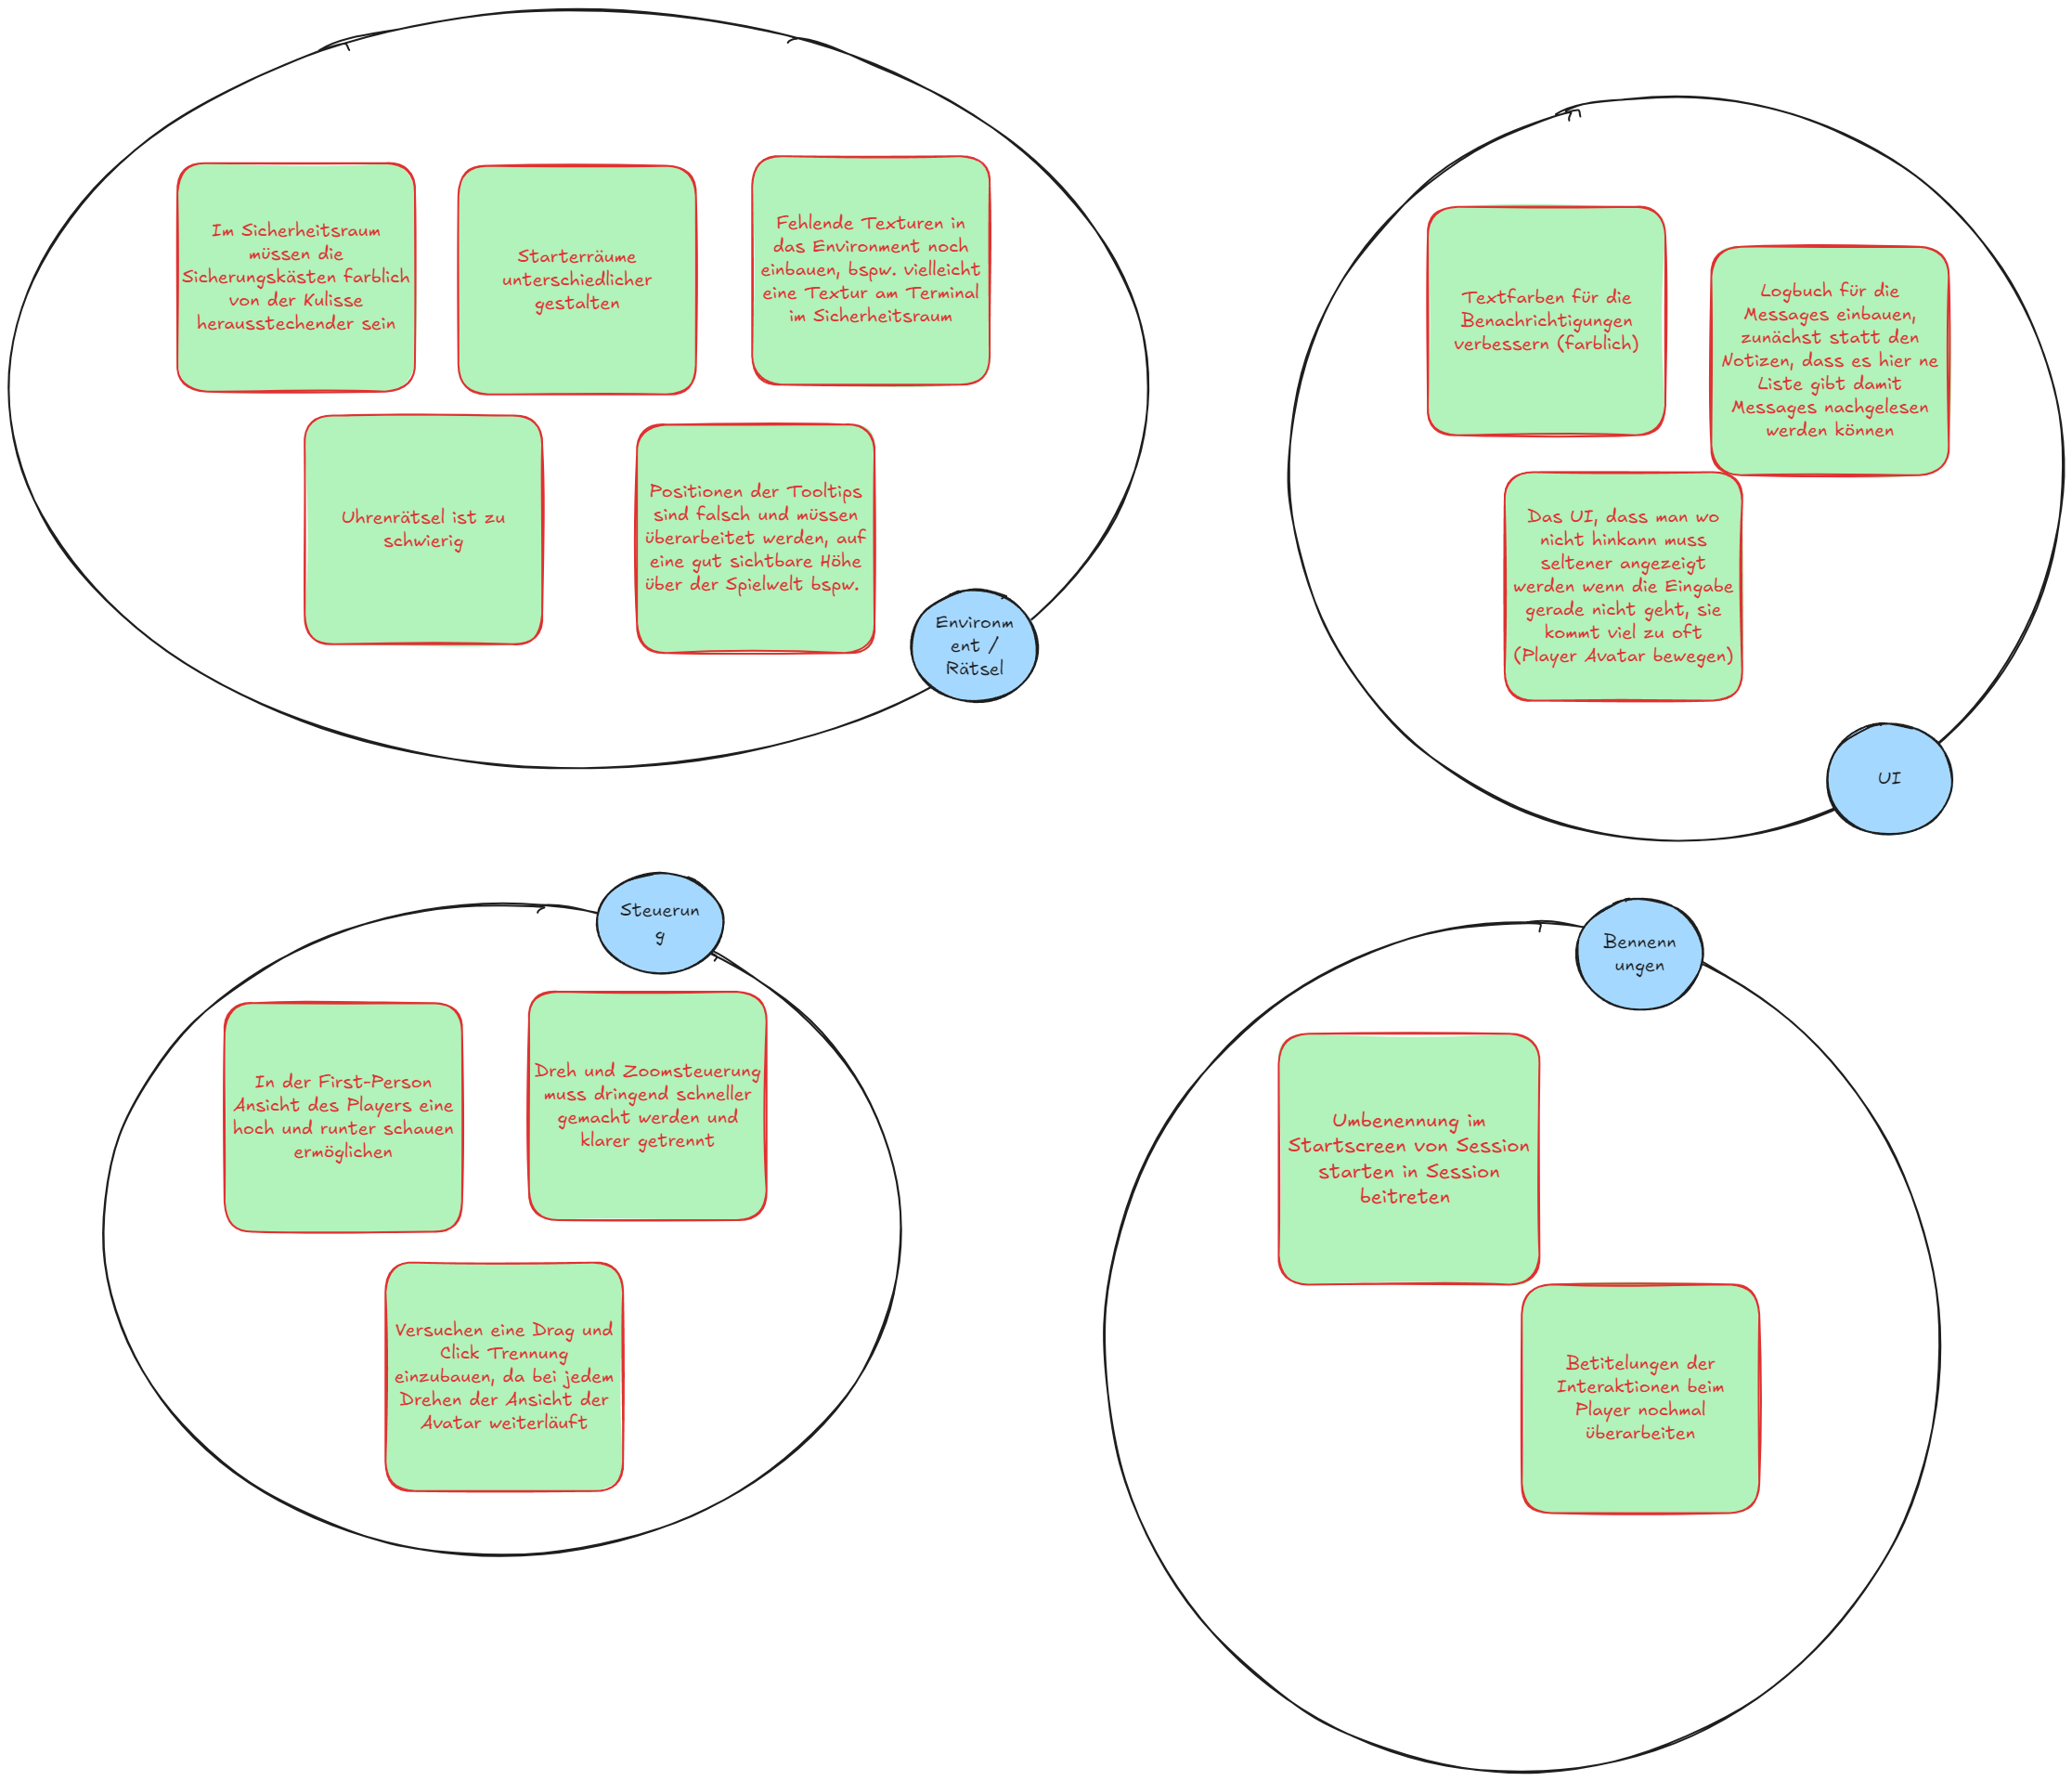
\includegraphics[width=1\linewidth]{content/pictures/Prestudy-Qualitative-Auswertung-Schritt-1.png}
\caption{Ergebnis der groben Kategorisierung nach \citealp{braun_using_2006} der Notizen aus Anhang \ref{sec:append_evaluation_pre_study_notes}: \nameref{sec:append_evaluation_pre_study_notes} (Quelle: eigene Darstellung)}
\label{fig:pre-study-qualitative-findings}
\end{figure}

Abbildung \ref{fig:pre-study-qualitative-findings} fasst die von den Teilnehmern geäußerten Aspekte zusammen. Ergänzt wurden diese um weitere Beobachtungen, die während der Tests auffielen, jedoch nicht explizit angesprochen wurden. Die gesammelten Aspekte lassen sich vier Hauptkategorien zuordnen:  Environmental / Rätsel, Steuerung, UI und Benennungen. In allen Bereichen wurden Verbesserungsvorschläge formuliert, die vor der Durchführung der groß angelegten Nutzerstudie umgesetzt werden sollten.

Besondere Relevanz kommt den Aspekten der Steuerung zu, insbesondere der Dreh- und Zoom-Funktion innerhalb der Watcher-Anwendung. Darüber hinaus benötigen das Rätsel im Sicherheitsraum sowie das Uhrenrätsel klarere Hinweise und Anpassungen in der Lösungsstruktur.

Weitere Punkte betreffen kleinere bis mittlere kosmetische Optimierungen zur Verbesser der Nutzererfahrung. So waren einige Tooltips nicht korrekt oberhalb der Raumwände positioniert. Auch gestalteten sich die Starträume zu ähnlich, was ihrer Unterscheidbarkeit erschwerte. Ferner bedürfen verschiedene Benennungen im Startbildschirm einer Überarbeitung, um Missverständnisse zu vermeiden.

Die Benutzeroberfläche der Nachrichtenanzeige weist zudem Verbesserungsbedarf in der Kontrastgestaltung von Hintergrund und Schrift auf. Für die Watcher-Anwendung wurde darüber hinaus ein Übersichtsmenü angeregt, in dem empfangene Nachrichten nachgelesen werden können.

In der Player-Anwendung fiel negativ auf, dass bei der Navigation des Avatars eine Fehlermeldung erscheint, wenn auf unerreichbare Bereiche geklickt wird. Das Navigieren sollte benutzerfreundlicher gestaltet werden.

\begin{figure}[ht]
\centering
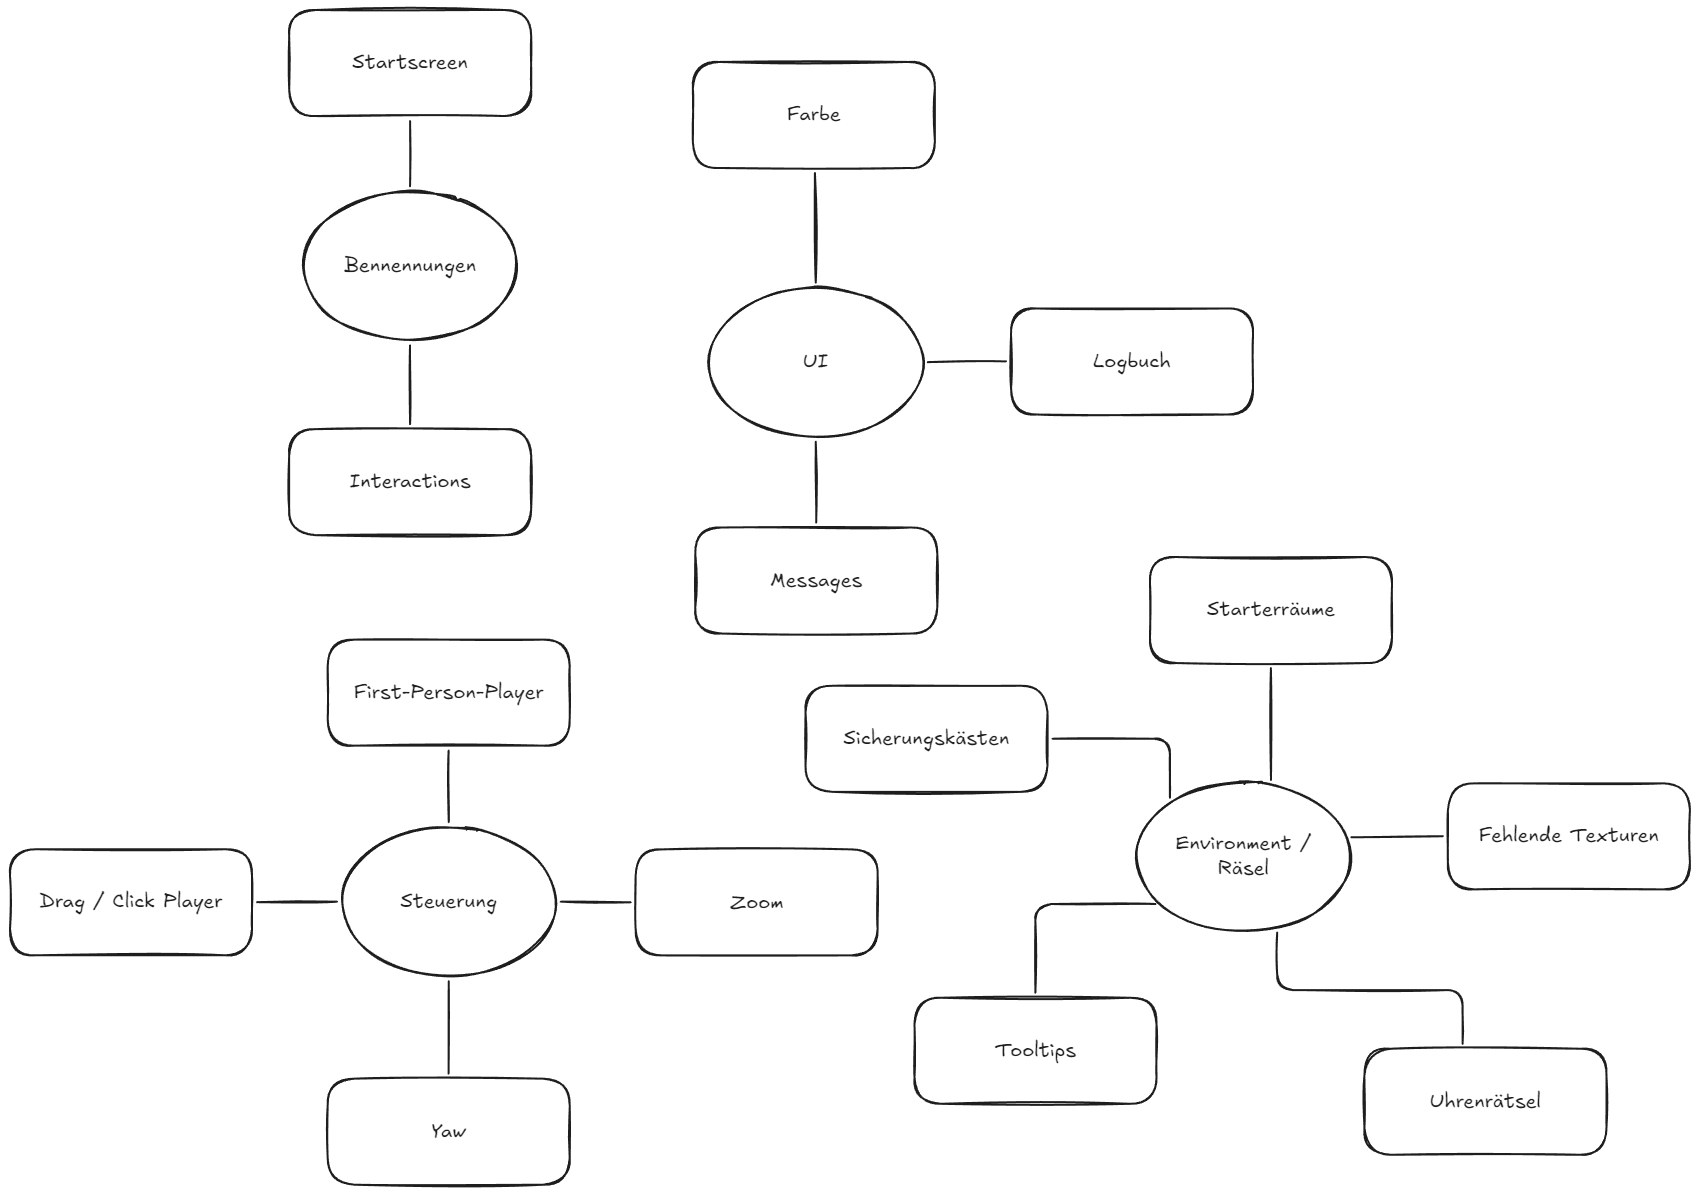
\includegraphics[width=1\linewidth]{content/pictures/Prestudy-Qualitative-Auswertung-Schritt-2.png}
\caption{Ergebnis der feinen Kategorisierung nach \cite{braun_using_2006} (Quelle: eigene Darstellung)}
\label{fig:pre-study-qualitative-findings_2}
\end{figure}

Eine detaillierte Kategorisierung der identifizierten Aspekte ist in Abbildung \ref{fig:pre-study-qualitative-findings_2} dargestellt.

\section{Handlungsempfehlungen}

Aus den gesammelten Ergebnissen lassen sich konkreten Handlungsempfehlungen ableiten, die vor der Durchführung der groß angelegten Nutzerstudie umgesetzt werden sollten.

Im Kontext der Verbesserung der Gebrauchstauglichkeit wurden diese Empfehlungen nach einem Severity Ranking priorisiert, wie in Abbildung \ref{fig:handlungsempfehlungen-vorstudie} dargestellt.

\begin{figure}[ht]
\centering
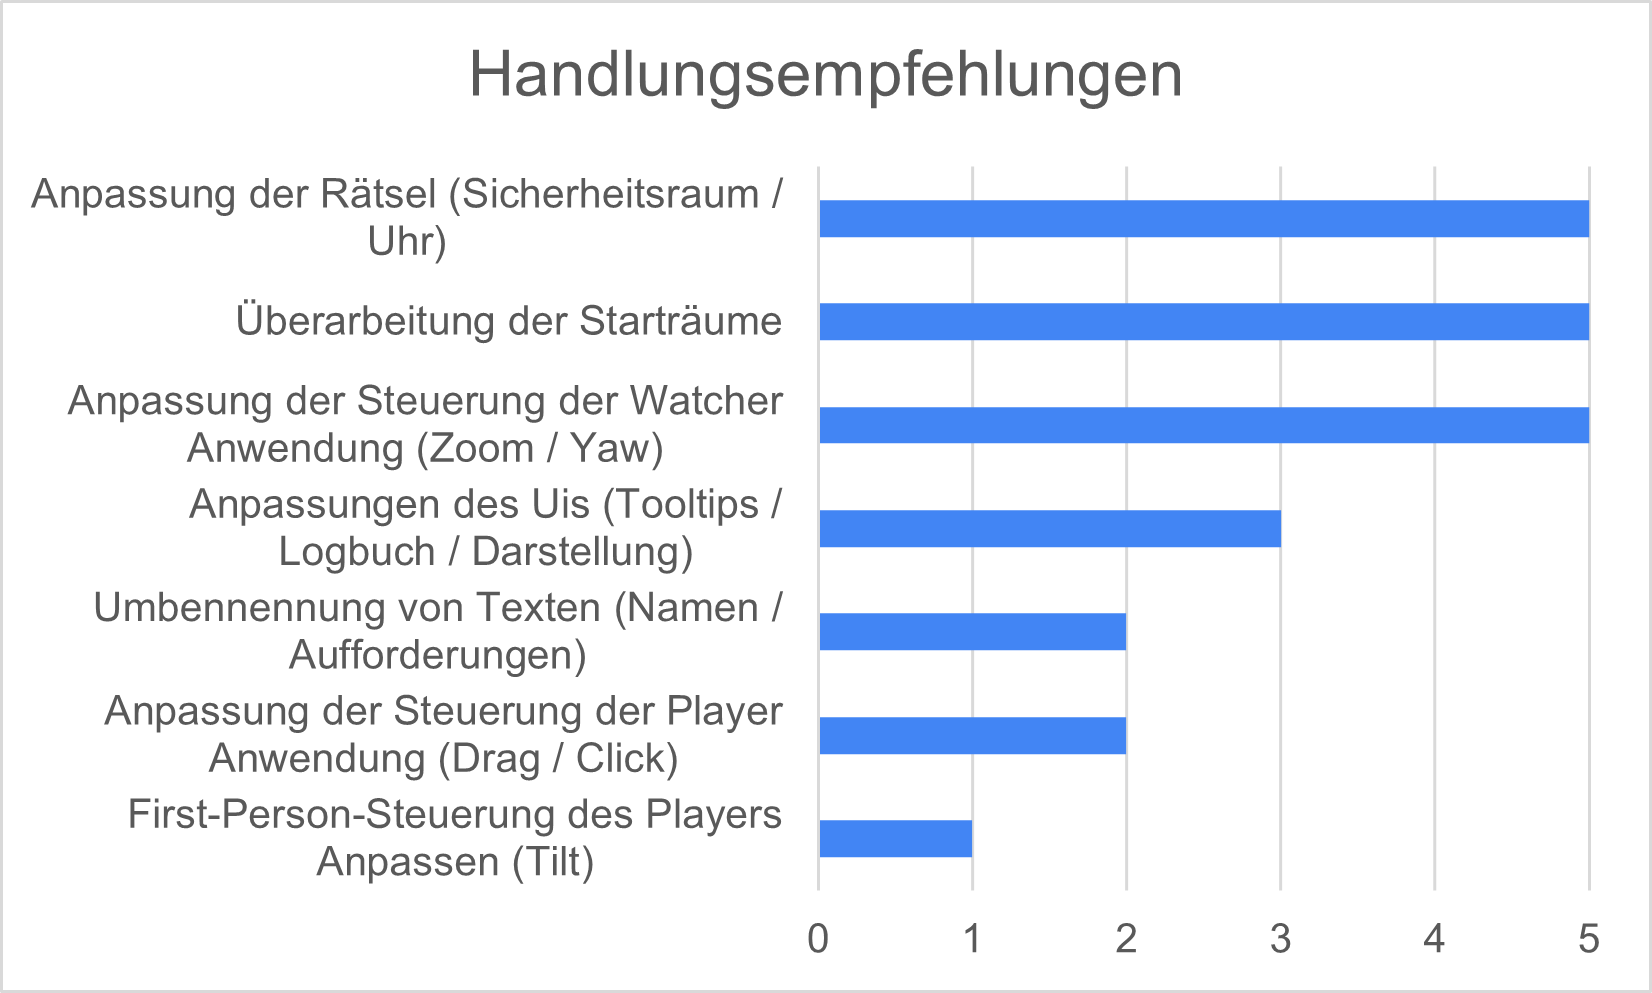
\includegraphics[width=1\linewidth]{content/pictures/Handlungsempfehlung_Vorstudie.png}
\caption{Handlungsempfehlungen zur Teststudie (Quelle: eigene Darstellung)}
\label{fig:handlungsempfehlungen-vorstudie}
\end{figure}

Besonders dringlich sind Anpassungen an der Steuerung der Watcher-Anwendungen, insbesondere im Hinblick auf die Dreh- und Zoomfunktion, da diese wiederholt als hinderlich wahrgenommen wurden. Ebenso kritisch sind Optimierungen an den Rätseln im Sicherheitsraum, sowie die Beseitigung eines Fehlers im Uhrenrätsel, da beide das Lösen der
Aufgaben unnötig erschwerten und zu Frustration führen könnte.

Ein weiterer zentraler Punkt betrifft die Gestaltung der Starträume. Diese müssen stärker differenziert werden, um den Einstieg in die Kommunikation einfacher zu gestalten. Momentan existieren nur Unterschiede in Form der Positionierungen der Fackeln und Schreibtischen. Der Einstieg ist von besonderer Relevanz, da das kommunikative Verhalten der Testpersonen im Zentrum der Gesamtstudie steht. In der bisherigen Testphase zeigten die Teilnehmer ein starkes Trial-and-Error-Verhalten, ohne sich ausreichend mit der Spielwelt auseinanderzusetzen. Dies könnte ein Hinweis auf mögliche Defizite in der Vermittlung zentraler Spielinformationen sein.

Darüber hinaus wurden verschiedene weniger schwerwiegende, aber dennoch relevante Mängel identifiziert. Dazu zählen kosmetische sowie funktionale Verbesserungen der Benutzeroberflächen, die Überarbeitung inkonsistenter oder unklarer Bezeichnungen sowie eine stärkere visuelle Trennung von \ac{UI}-Elementen und Hintergrund. Auch die Player-Anwendung könnte von Verbesserungen profitieren, bspw. durch eine überarbeitete Rückmeldung bei nicht erreichbaren Navigationszielen. Diese Aspekte besitzen jedoch im Vergleich zu den zuvor genannten Punkten eine geringe Priorität für den Gesamterfolg der Anwendung.

Abschließend wird empfohlen eine weitere Zwischentestphase durchzuführen, um die umgesetzten Maßnahmen auf ihre Wirksamkeit zu überprüfen. Eine solche Zwischenevaluation ermöglicht eine fundierte Einschätzung der verbleibenden Mängel und schafft die Grundlage für eine erfolgreiche Durchführung der abschließenden Nutzerstudie.

\section{Zusammenfassung und Interpretation der Ergebnisse}

Die identifizierten Schwerpunkte betreffen primär die Steuerungsmechaniken der Watcher- und Player-Anwendungen. Darüber hinaus wurden Aspekte des gestaltete Environments sowie der implementierten Rätsel als überarbeitungsbedürftig eingestuft. Besonders im Bereich der Benutzeroberfläche traten Darstellungsprobleme einzelner \say{UI}-Elemente auf, die entweder nicht an der vorgesehenen Position angezeigt wurden, oder eine visuelle Überarbeitung benötigen. Zusätzlich führten unklare oder uneinheitliche Benennungen von Aktionen und Menüpunkten zu Verwirrung bei den Testpersonen, weshalb auch hier Anpassungen erforderlich waren.

Insgesamt bieten die Ergebnisse wichtige Hinweise auf bestehende Mängel im Prototyp, die vor der nächsten Testphase behoben werden sollten. Gleichzeitig ist der Umfang der identifizierten Probleme vergleichsweise gering, was für eine frühe Testphase als positives Indiz zu werten ist. Dies lässt darauf schließen, dass in der bisherigen Entwicklungsphase ein hoher Grad an internen Tests stattgefunden hat, durch die potenzielle Fehlerquellen und Edge-Cases bereits weitestgehend identifiziert und reduziert werden konnten.

\section{Methodendiskussion}

Wie bereits in Kapitel \ref{sec:analysis-discussion} angesprochen, wird auch an dieser Stelle die angewandte Methodik kritisch reflektiert.

Zunächst ist die Wahl der Methodik und die daraus resultierende Erkenntnisqualität zu betrachteten. Die Kombination aus Thinking-Aloud-Methode und begleitender Beobachtung der Probanden ermöglichte einen ersten fundierten Einblick in die Nutzung der Anwendungen. Die dabei dokumentierten Eindrücke lieferten qualitative Hinweise auf bestehende Schwächen, die im weiteren Verlauf der Arbeit adressiert werden müssen. Der Vorteil dieser Vorgehensweise liegt in der Fokussierung auf ein vertieftes Verständnis der Nutzerwahrnehmung, das über einen rein quantitatives Messwert hinausgeht. Allerdings ist die fehlende Erhebung quantitativer Daten auch als Limitation zu bewerten, da dadurch die wissenschaftliche Vergleichbarkeit und Messbarkeit der Ergebnisse eingeschränkt ist.

Im weiteren Verlauf wird die zeitliche Einbettung der Vorbereitungstests in den Gesamtprozess der Studienplanung betrachtet. Die Tests fanden lediglich einen Tag vor der eigentlichen Nutzerstudie statt. Idealerweise sollte eine solche Vorbereitungsphase mehrere Wochen vor dem Haupttest durchgeführt werden, um ausreichend Zeit für die Umsetzung des Feedbacks zu gewährleisten. Ein Großteil der verfügbaren Zeit wurde in die Entwicklung der Rätsel und der Anwendungen selbst investiert, ohne frühzeitig externe Testpersonen einzubinden. Hierbei ist jedoch die technische Komplexität des Setups zu berücksichtigen. Um Tests in einem digitalen Format zu ermöglichen, hätte die Server-Infrastruktur (inklusive Docker-Container) extern gehostet werden müssen. Aufgrund fehlender Ressourcen war die nicht möglich, sodass die Tests lokal vor Ort durchgeführt werden mussten, was eine sorgfältige Planung von Hardware und Räumlichkeiten erforderte.

Ein weiterer relevanter Aspekt betrifft, wie bereits in Kapitel \ref{sec:pre-study-sample} dargelegt, die Auswahl der Probanden. Die Teilnehmer der Vorbereitungstest durften nicht an der eigentlichen Nutzerstudie teilnehmen, um eine Beeinflussung der Ergebnisse zu vermeiden. Daher wurden Personen rekrutiert, die bereits mit dem Projekt vertraut waren. Für den angestrebten Zweck, das Aufdecken grundlegender Gebrauchstauglichkeitsprobleme, war diese Auswahl angemessen. Auch die Anzahl der Teilnehmer erwies sich als ausreichend, um erste zentrale Schwächen zu identifizieren. Dennoch wäre es wünschenswert gewesen, bereits in der Entwicklungsphase mehrere Testzyklen durchzuführen, um wiederkehrende oder tiefgreifende Probleme frühzeitig zu erkennen und gezielt adressieren zu können.

Abschließend ist die technische Infrastruktur der Anwendungen zu reflektieren. Wie bereits beschrieben, musste die Testphase in Präsenz erfolgen. Die dafür notwendige Hardware musste zunächst organisiert und bereitgestellt werden. Im Verlauf zeigte sich, dass nicht alle technischen Anforderungen im Vorfeld ausreichend berücksichtigt worden waren. Insbesondere erschwerte eine Netzwerksicherheitsmaßnahme der Hochschule die geplante Kommunikation der Geräte im lokalen Netzwerk. Durch die exakte Vorbereitung der Testphase konnte jedoch rechtzeitig eine Lösung gefunden werden, sodass sowohl die Vorabtests als auch die eigentliche Nutzerstudie wie vorgesehen durchgeführt werden konnte.

Zusammenfassend ist festzuhalten, dass die Vorbereitungstests in größerer Zahl und mit einem größeren zeitlichen Vorlauf hätten stattfinden sollen. Dies hätte zur frühzeitigeren Identifikation kritischer Gebrauchstauglicher-Probleme beigetragen und die Qualität der nachfolgenden Nutzerstudie weiter verbessert.











\chapter{Evaluation des Prototyps sowie der Wirkung des Prototyps auf das Kommunikationsverhalten der Probanden} \label{sec:study}

Dieser Abschnitt widmet sich der Evaluation der entwickelten Anwendungen sowie der Überprüfung ihrer intendierten Wirkung. Im Fokus steht dabei die Identifikation von Elementen des Prototyps, die weiterentwickelt werden müssen. Zugleich liefert die Auswertung erste Erkenntnisse über die Effektivität der Anwendung im Hinblick auf die angestrebten Ziele.


\section{Methodik}

In der dritten Testphase steht die Evaluationen der entwickelten Anwendungen im Fokus, insbesondere im Hinblick auf deren Wirkung im Kontext der Kommunikationsforschung zu asymmetrischen Multiplayerspielen. Untersucht werden sowohl die kommunikative Effektivität der Anwendungen als auch ihre funktionale und gestalterische Gebrauchstauglichkeit. Die getesteten Anwendungen basieren auf den zuvor entwickelten Konzepten sowie den Optimierungen, die aus der vorangegangenen Testphase abgeleitet wurden.

Zur Erhebung der relevanten Daten kommt eine kombinierte Methodik zum Einsatz, die qualitative und quantitative Verfahren innerhalb eines experimentellen Studiensettings miteinander verbindet. Ziel ist es, ein möglichst umfassendes Bild der Nutzung und der Interaktion mit der Anwendung zu gewinnen.

\subsection{Forschungsdesign}

Zur Untersuchung der Forschungsfragen  \say{Welche Verbesserungen in der Kommunikation zwischen den Anwendern können durch ein asymmetrisches Multiplayer-Spiel mit zwei verschiedenen Spielerklassen beobachtet werden?} sowie \say{Wie stehen die Nutzer zu einem spielerischen Ansatz und zur Verbesserung der Kommunikation, insbesondere auch im Umgang mit Fremden?} wurde ein praxisorientiertes, experimentelles Forschungsdesign gewählt. Im Zentrum steht ein asymmetrisches Multiplayer-Szenario, in dem jeweils zwei Personen unterschiedliche Rollen mit ungleich verteilten Informationen übernehmen. Diese Konstellation ermöglicht es, die Auswirkungen der Anwendungen auf kooperative Kommunikationsprozesse zu trainieren und in Form einer Prüfungsumgebung gezielt zu analysieren.

Das gewählte Studiendesign kombiniert quantitative und qualitative Erhebungsverfahren, um sowohl messbare Effekte als auch subjektive Wahrnehmungen und Erfahrungen der Teilnehmer zu erfassen.

\subsection{Erhebungsinstrumente}

Die Datenerhebung dieser Studie erfolgt mittels standardisierter Fragebögen, die sowohl Usability, Spielerlebnis, mentale Beanspruchung als auch affektive und zwischenmenschliche Aspekte erfassen.

Zur Evaluation der Gebrauchstauglichkeit der Anwendungen wurde der \ac{SUS} (vgl. \citealp{brooke_sus_1995}) eingesetzt. Das Spielerlebnis wurde mit dem \ac{GEQ} (vgl. \citealp{ijsselsteijn_game_2013}) erfasst und durch die Subskalenbereiche \say{Interesse/Vergnügen} des \ac{IMI} (vgl. \citealp{mcauley_psychometric_1989}) ergänzt. Die wahrgenommene mentale Beanspruchung während der Nutzung wurde mit dem \ac{NASA-TLX} (vgl. \citealp{hart_nasa-task_2006}) erfasst.

Zur Messung des affektiven Zustands der Probanden zu Beginn und am Ende des Tests wurde der \ac{SAM} (vgl. \citealp{russell_evidence_1977}) verwendet, welcher die Dimensionen Valenz, Erregung und Dominanz abbildet. Diese Zustände können potenziell Einfluss auf die Qualität der Kommunikation nehmen.

Zur Einschätzung der sozialen Nähe zwischen den Teilnehmern kam  zu Beginn und am Ende der \ac{IOS} (vgl. \citealp{gachter_measuring_2015}) zum Einsatz. Ergänzend wurde am Ende ein Fragebogen zur Rollenverteilung in Miteinander nach \cite{emmerich_game_2016} eingesetzt, um Hinweise auf Führungsverhalten innerhalb der Interaktionen zu gewinnen (vgl. \citealp[S. 5]{emmerich_game_2016}). Zudem wurde der \ac{QCAE} (vgl. \citealp{reniers_qcae_2011}) ausgefüllt, um die kognitive Empathie der Teilnehmer zu erfassen.

Im Fokus der Studie stehen damit insbesondere die soziale Nähe, das emotionale Empfinden und die empathischen Fähigkeiten der Teilnehmer. Faktoren, die in der kommunikativen Interaktion eine zentrale Rolle spielen. Ziel ist es Rückschlüsse darauf zu ziehen, wie die Variablen der Qualität und Effektivität die Kommunikation beeinflussen.

Zusätzlich wurde ein eigens entwickelter Fragebogen eingesetzt, um die Haltung der Teilnehmer zum Spielen mit fremden Personen zu erfassen. Auch ein demografischer Fragebogen wurde speziell für die Zielsetzung dieser Arbeit erstellt. Zur Einordnung individueller Spielvorlieben ordneten sich die Probanden einem der vier Spielertypen nach  \cite{bartle_hearts_1996} zu. Diese Taxonomie wurde gewählt, da sie trotz geringer Stichprobengröße eine grundlegende Gruppierung erlaubt, die für Interpretation der Kommunikationstypen ausreichend differenzierend ist.

Zur Analyse der tatsächlichen Kommunikation wurden alle Versuchsdurchführungen aufgezeichnet (vgl. Anhang \ref{sec:append_study_protocols}: \nameref{sec:append_study_protocols}). Die Auswertung erfolgt auf Grundlage der Methoden von \cite{nasir_cooperative_2013,nasir_effect_2015}, welche den Kontrollfluss in der Kommunikation quantifiziert. Diese Methode erlaubt Rückschlüsse auf dominante Sprechanteile, Gesprächsfluss und potenzielle Dysbalancen in der Kommunikation, wie etwa Pausen oder Unterbrechungen. Sie ist besonders geeignet, um asymmetrische Kommunikationsverhältnisse sichtbar zu machen.

Die Kombination qualitativer und quantitativer Verfahren erlaubt somit eine umfassende Analyse der Wirkung der Anwendung, sowohl im Hinblick auf objektive Veränderungen in der Gesprächsstruktur als auch auf die subjektive Wahrnehmung der Interaktion und Kommunikation durch die Teilnehmer.

\subsection{Stichprobe}

Die Festlegung der Stichprobengröße orientierte sich sowohl an den quantitativen als auch den qualitativen Zielsetzungen der Studie. Die für quantitative Analyse wurde das Signifikanzniveau auf $\alpha = 0,05$ festgelegt. Nach \cite{cohen_power_1992} ist eine Stichprobengröße von mindestens 28 Personen erforderlich, um verlässliche Ergebnisse in Signifikanztests zu erzielen (vgl. \citealp[S. 158]{cohen_power_1992}). Dies entspricht 14 Dyaden.

Aus qualitativer Perspektive, kann wie bereits in Kapitel \ref{sec:pre-study-sample} erwähnt, eine Stichprobengröße von sieben Probanden ausreichen, um alle Aspekte der Gebrauchstauglichkeit zu identifizieren. Vor diesem Hintergrund wurde eine Stichprobengröße von insgesamt 14 Personen bzw. sieben Dyaden gewählt. Dieses Entscheidung berücksichtigt neben methodischen Anforderungen auch praktische Rahmenbedingungen wie die freiwillige Teilnehmerbereitschaft, den zeitlichen Umfang der Datenerhebung sowie den Auswertungsaufwand, insbesondere im Hinblick auf die Transkription der gesprochenen Interaktion.

Damit wurde ein ausgewogener Kompromiss zwischen wissenschaftlicher Fundierung und praktischer Umsetzbarkeit geschaffen, der valide und aussagekräftige Ergebnisse ermöglicht.

\subsection{Durchführung der Studie}

Die Rekrutierung der Probanden erfolgte über Einladungsnachrichten in verschiedene Chatgruppen sowie über mehrere Rundmails. Interessierte konnten sich eigenständig über eine Terminkalender-Anwendung in einen verfügbaren Zeitslot für den Probandentest eintragen.

Zu Beginn des Tests wurden die Teilnehmer begrüßt und gebeten, eine Einverständniserklärung (vgl. Anhang \ref{sec:append_study_consent}: \nameref{sec:append_study_consent}) zu unterzeichnen, da während des Versuchsdurchlaufs Videoaufzeichnungen vorgenommen wurden. Der genaue Zweck der Studie wurde den Probanden zu diesem Zeitpunkt bewusst nicht mitgeteilt. Sie wurden lediglich darüber informiert, dass sie an einem asymmetrischen Multiplayerspiel teilnehmen würden, in dem sie gemeinsam im Team Rätsel lösen und dabei unterschiedliche Rollen einnehmen sollen.

Diese Form der partiellen Informationszurückhaltung diente dem Zweck, Verzerrungen in der Datenerhebung zu vermeiden. Eine informierte Vorannahme über Ziel und Aufbau des Experiments hätte möglicherweise zu einer Beeinflussung des natürlichen Spielverhaltens geführt. Die methodische Vorgehensweise orientierte sich an dem bekannten Milgram-Experiment (vgl. \citealp{milgram_behavioral_1963}), bei dem ebenfalls auf eine vollständige Aufklärung im Vorfeld verzichtet wurde, um die Validität der Ergebnisse zu gewährleisten. Die Teilnehmenden erhielten ausschließlich konkrete Handlungsanweisungen zu den im Verlauf zu bearbeitenden Aufgaben.

Vor Beginn des eigentlichen Versuchsablaufs füllten die Probanden einen demografischen Fragebogen aus, der Information zu Alter, Geschlecht sowie Vorerfahrungen mit digitalen Spielen, Multiplayerspielen und Touchsteuerung erfasste (vgl. Anhang \ref{sec:append_study_demografic}: \nameref{sec:append_study_demografic}). Im Anschluss wurden standardisierte Fragebögen zur wechselseitigen Beziehung zwischen den Spielern (vgl. Anhang \ref{sec:append_study_ios}: \nameref{sec:append_study_ios}), zur Einordnung des Spielertyps nach Bartle (vgl. Anhang \ref{sec:append_study_bartle}: \nameref{sec:append_study_bartle}) sowie zur Erhebung des aktuellen affektiven Zustands ausgefüllt (vgl. Anhang \ref{sec:append_study_sam}: \nameref{sec:append_study_sam}).

Die eigentliche Versuchsdurchführung gliederte sich in drei Hauptkomponenten. Den Kern bildete das Spielen des entwickelten Prototyps, das zwischen einem Vor- und einem Nachtest stattfand.

Zunächst absolvierten die Teilnehmer den Vortest.

\begin{figure}[ht]
\centering

\includegraphics[width=0.3\linewidth]{content/pictures/MazeScape.jpg}
\caption{Verpackung des Spiels MazeScape (Quelle: \citealp{cespedes_mazescape_2023})}
\label{fig:mazescape}
\end{figure}

\begin{figure}[ht]
\centering

\includegraphics[width=0.5\linewidth]{content/pictures/MazeScape_Level02.jpg}
\caption{Level 02 aus dem Spiel MazeScape (Quelle: \citealp{cespedes_mazescape_2023})}
\label{fig:mazescape_level-02}
\end{figure}

Der Vortest bestand im Spielen des zweiten Levels (vgl. Abbildung \ref{fig:mazescape_level-02}) aus dem physischen Spiel \say{MazeScape} )vgl. Abbildung \ref{fig:mazescape}), dessen allgemeine Spielmechanik der Navigation durch ein Labyrinth für den vorliegenden Untersuchungszweck übernommen wurde. Spezifische Spielregeln, etwa zu Gegenständen, Punktesystemen oder Gegnern wurden aufgrund ihrer fehlenden Relevanz für die Studie nicht berücksichtigt.

Die Probanden hatten zehn Minuten Zeit, um gemeinsam mit einer Spielfigur vom Startpunkt das Ziel des Labyrinths zu erreichen. Das Erreichen des Ziels innerhalb der vorgegebenen Zeit war dabei nicht zwingend erforderlich.

Ziel dieses Vortests war es, einen Ausgangswert der kommunikativen Interaktion zwischen den Teilnehmern zu erfassen, um diesen später mit den Ergebnissen des Nachtests vergleichen zu können. Es wurde erwartet, dass sich die Kommunikation durch das gemeinsame Lösen der Aufgaben im anschließenden Test verbessern würde.

Unabhängig vom erfolgreichen oder nicht erfolgreichen Abschluss des Vortests erfolgte im Anschluss die Erprobung des Prototyps Connecting-Minds. Vor Beginn erhielten die Teilnehmenden eine Einführung in die jeweilige Steuerung ihrer Anwendung. Danach startete der Testlauf, für den 40 Minuten zur Verfügung standen. Ziel war es, gemeinsam die vorgesehenen Rätsel zu lösen. Ein vollständiger Abschluss des Tutorials innerhalb der Zeitvorgabe war nicht erforderlich.

Die Zuweisung der Spielerrollen erfolgte unmittelbar nach der Begrüßung durch die Probanden selbst. Da für die ersten Fragebögen relevant war, welche Person welche Rolle im Spiel übernahm, wurde diese Information bereits beim Ausfüllen der Einverständniserklärung dokumentiert.

Nach Abschluss des Spielens mit dem Prototyp bearbeiteten die Teilnehmer mehrere standardisierte Fragebögen. Diese umfassten Aspekte der System Usability (vgl. Anhang \ref{sec:append_study_sus}: \nameref{sec:append_study_sus}), der Spielerfahrung (vgl. Anhang \ref{sec:append_study_xp}: \nameref{sec:append_study_xp}) und Motivation (vgl. Anhang \ref{sec:append_study_imi}: \nameref{sec:append_study_imi}) sowie des individuell wahrgenommenen Workloads (vgl. Anhang \ref{sec:append_study_tlx}: \nameref{sec:append_study_tlx}).

Im Anschluss daran fand der Nachtest statt. Hierzu spielten die Probanden ein weiteres Level aus dem Spiel MazeScape, konkret das Level drei (vgl. Abbildung \ref{fig:mazescape_level-03}). Wie bereits im Vortest, wurden lediglich die grundlegenden Regeln zur Fortbewegung innerhalb der Spielwelt mitgeteilt. Weiterführende Spielregeln etwa zu Gegenständen oder Gegnern blieben auch hier unberücksichtigt.

Eine zusätzliche Herausforderung in diesem Level bestand darin, dass die Teilnehmer zunächst gemeinsam das Ziel innerhalb des Labyrinths lokalisieren mussten, bevor sie einen geeigneten Weg dorthin finden konnten.

\begin{figure}[ht]
\centering

\includegraphics[width=0.5\linewidth]{content/pictures/MazeScape_Level03.jpg}
\caption{Level 03 aus dem Spiel MazeScape (Quelle: \citealp{cespedes_mazescape_2023})}
\label{fig:mazescape_level-03}
\end{figure}

Wie bereits im Vortest stand den Probanden auch im Nachtest ein Zeitraum von zehn Minuten zur Verfügung. Ein erfolgreiches Erreichen des Ziels innerhalb dieser Zeit war erneut nicht zwingend erforderlich.

Nach Abschluss der Tests wurden abschließend weitere Fragebögen ausgefüllt. Diese dienten der Erhebung von Vergleichswerten zur wechselseitigen Beziehung zwischen den Teilnehmern sowie zur Erfassung des affektiven Status nach der gemeinsamen Spielerfahrung. Darüber hinaus beantworteten die Probanden Fragebögen zu den Themen Leadership (vgl. Anhang \ref{sec:append_study_leader}: \nameref{sec:append_study_leader}) sowie zwischenmenschlichen Umgang im Rahmen des Versuchsaufbaus. Abschließend bestand die Möglichkeit, im Rahmen eines Freitextfeldes individuelles qualitatives Feedback zur Anwendung und/ oder dem Versuch zu geben.

Nach dem Ausfüllen aller Fragebögen wurde die Videoaufzeichnung beendet, welche zum Start des Vortests gestartet wurde. Den Teilnehmern wurde für ihr Mitwirken gedankt und sie konnten sich an den bereitgestellten Snacks bedienen. Anschließend wurden sie aus der Untersuchung entlassen.

Die gesamte Versuchsdurchführung nahm pro Dyade etwa 75 Minuten in Anspruch.

\subsection{Rahmenbedingungen}

Für die Durchführung des Versuchsaufbaus wurde der Seminarraum im I-Bau der ehemaligen Fakultät \ac{DM} reserviert.

Im Unterschied zu den Rahmenbedingungen der zuvor beschriebenen Probandentests (vgl. Kapitel \ref{sec:pre-study-rahmen}) wurden die Versuchsdurchläufe in diesem Fall mithilfe der Sony Kamera auf dem Stativ videografisch dokumentiert.

\begin{figure}[ht]
\centering
\includegraphics[width=0.8\linewidth]{content/pictures/Aufbau_00.jpg}
\caption{Versuchsaufbau des Experiments (Quelle: eigene Darstellung)}
\label{fig:study-experiment-00}
\end{figure}

\begin{figure}[ht]
\centering
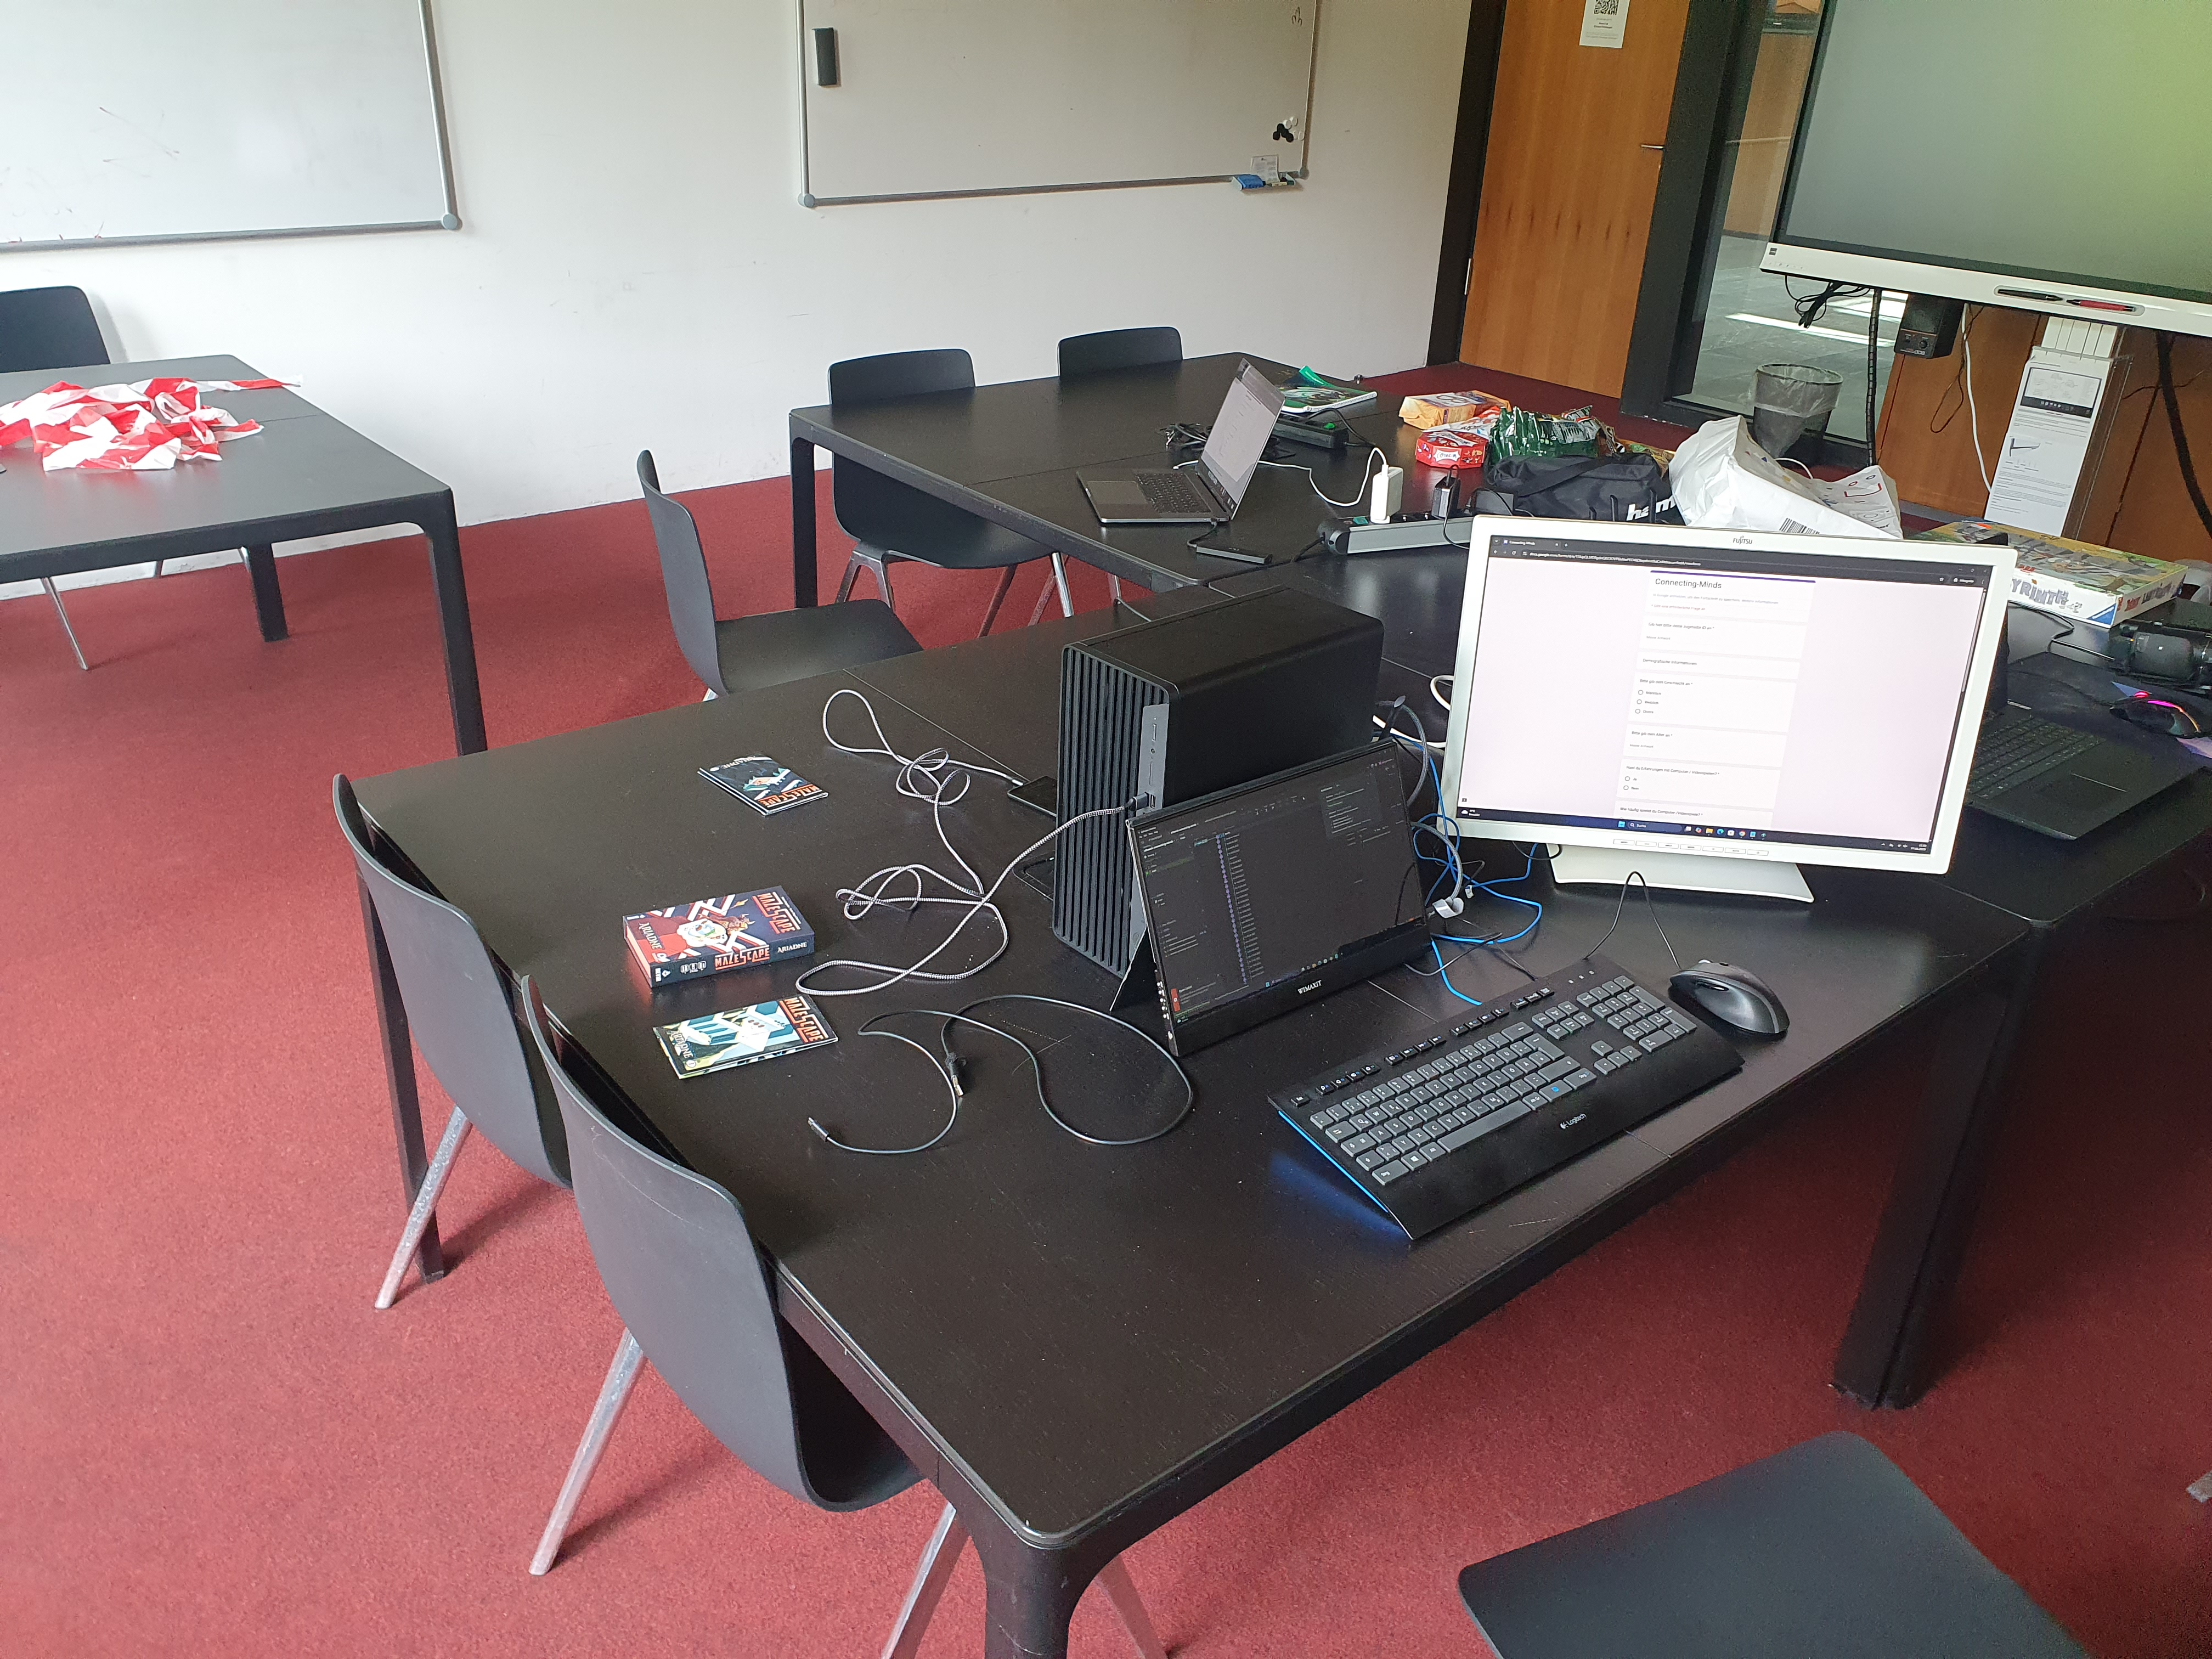
\includegraphics[width=0.8\linewidth]{content/pictures/Aufbau_01.jpg}
\caption{Versuchsaufbau Seite des Players (Quelle: eigene Darstellung)}
\label{fig:study-experiment-01}
\end{figure}

\begin{figure}[ht]
\centering
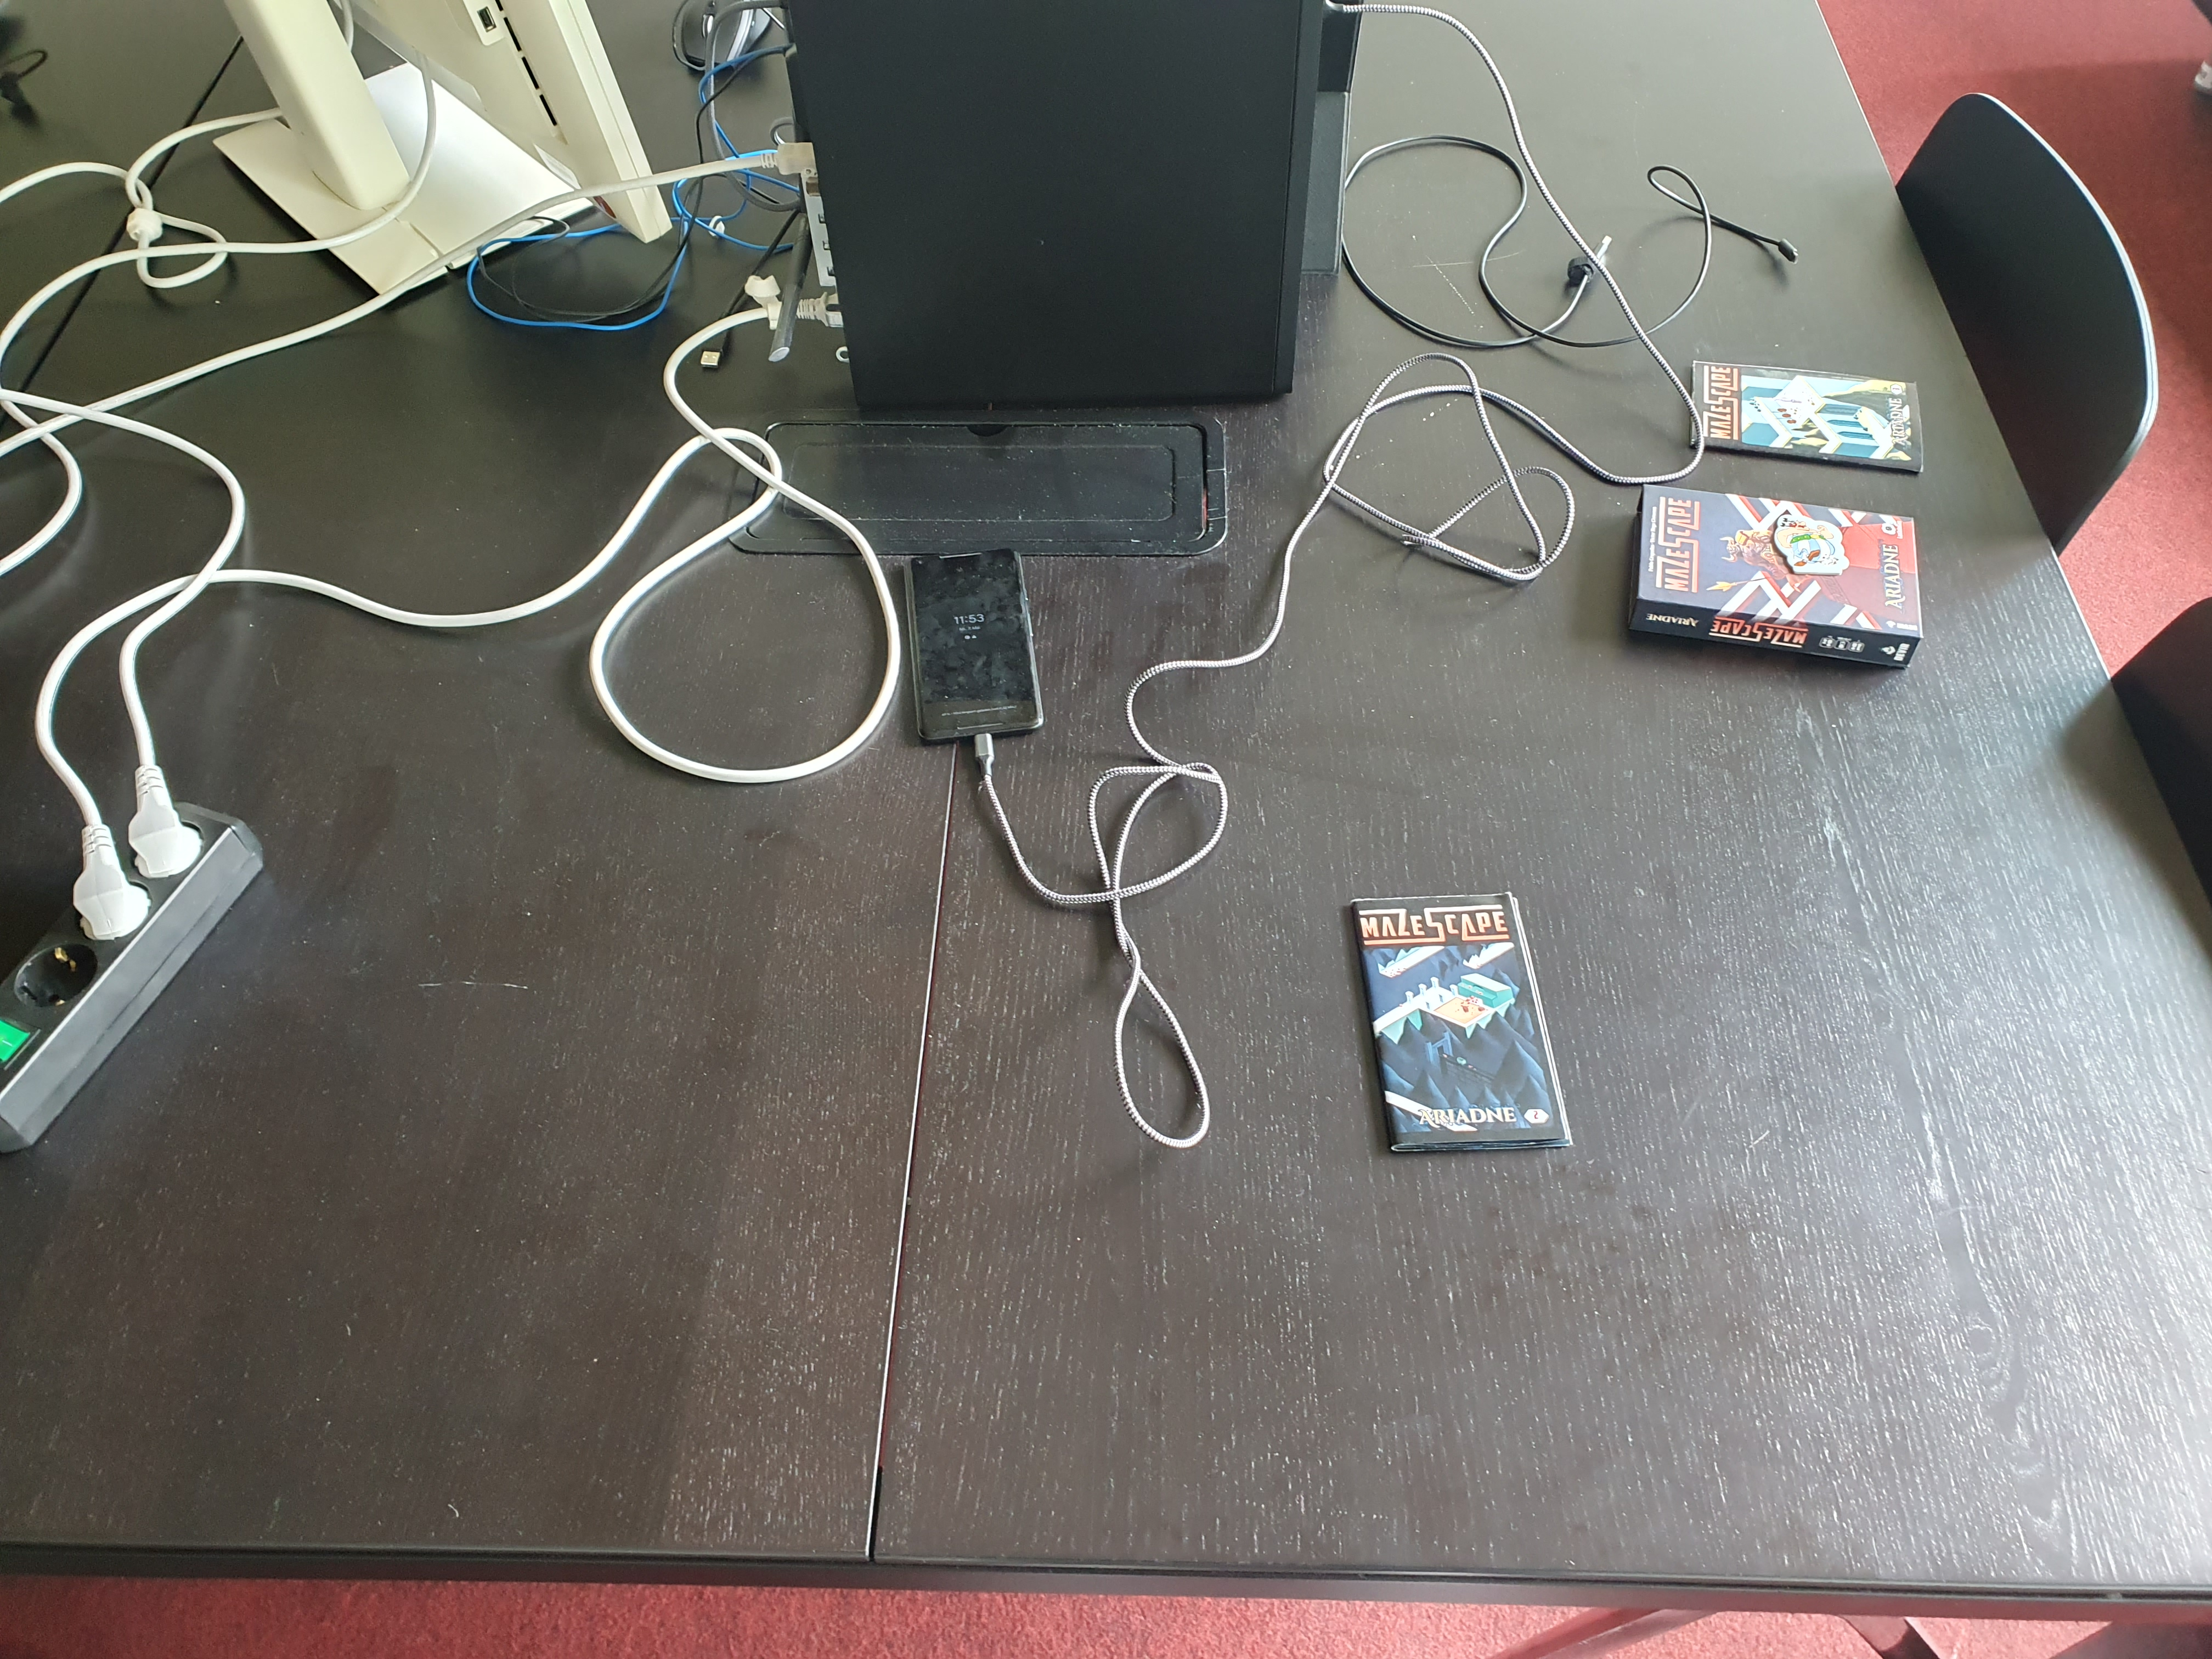
\includegraphics[width=0.8\linewidth]{content/pictures/Aufbau_02.jpg}
\caption{Versuchsaufbau Seite des Watchers (Quelle: eigene Darstellung)}
\label{fig:study-experiment-02}
\end{figure}

Abbildung \ref{fig:study-experiment-00} zeigt die Anordnung des Seminarraums während der Versuchsdurchführung. Die beiden Spielteilnehmern saßen sich an einem quadratischen Tisch gegenüber. Zwischen ihnen war der Rechner für die Player-Anwendung positioniert, der zugleich als  physische Barriere diente. Diese räumliche Trennung war von zentraler Bedeutung, um zu verhindern, dass die Probanden in die Anwendung der jeweils anderen Person blicken und dadurch Aufgaben lösen konnten, ohne miteinander zu kommunizieren. Ein Blick in die Anwendung der anderen Person war ausdrücklich untersagt. 

Auf der rechten Seite des Tisches befand sich der Platz des Players (vgl. Abbildung \ref{fig:study-experiment-01}). Dieser steuerte seine Anwendung über einen Touchmonitor, der sich direkt vor ihm befand. Zusätzlich erhielt er für das Ausfüllen der Fragebögen im Rahmen der Versuchsdurchführung eine Tastatur sowie eine Maus und einen großen Bildschirm.

Der Watcher nahm auf der linken Seite des Tisches Platz (vgl. Abbildung \ref{fig:study-experiment-02}). Dort nutzte er das bereitgestellte Google Pixel, um die Watcher-Anwendung, die umgesetzte \ac{3D}-Anwendung zu bedienen. In diesem Bereich fanden auch der Vor- und Nachtest statt. Die Probanden konnte wählen, ob er sich im sitzen oder stehen durch das Labyrinth navigieren wollte.


Am linken Bildrand von Abbildung \ref{fig:study-experiment-00} ist ein weiterer Laptop zu sehen, über den der Watcher seine Fragebögen ausfüllte.

\section{Ergebnisse}

In diesem Kapitel werden die Ergebnisse der verschiedenen Fragebögen sowie der Videoaufzeichnung der Versuchsdurchführungen dargestellt. Die Präsentation der Ergebnisse erfolgt thematisch gegliedert in einzelnen Unterabschnitten, orientiert am jeweiligen inhaltlichen Schwerpunkt.

\subsection{Vorstellung der demographischen Daten}

An der Versuchsdurchführung nahmen insgesamt N = 14 freiwillige Probanden teil (3 weiblich, 11 männlich; M = 25,86; SD = 4,52 Jahre). Daraus ergaben sich sieben Dyaden für die Durchführung der Studie. Zwei Teilnehmer kannten sich zu Beginn der Untersuchung nicht bzw. lediglich flüchtig. 

Zwölf der Probanden gaben an, bereits Erfahrungen mit Video- und Computerspielen gesammelt zu haben; zwei Personen verfügten über keine diesbezüglichen Vorerfahrungen. Hinsichtlich der durchschnittlichen wöchentlichen Spielzeit ergab sich folgendes Bild: fünf Personen spielen mehr als 10 Stunden pro Woche, drei zwischen 6-10 Stunden, 
jeweils zwei zwischen 3-5 bzw. 1-2 Stunden und zwei gaben an, keine Zeit mit digitalen Spielen zu verbringen.

Bezüglich der Erfahrung mit Multiplayerspielen bestätigten 13 Teilnehmer entsprechende Vorerfahrungen, während eine Person angab, keine Multiplayer-Erfahrung zu haben. Drei Teilnehmer spielen mehr als 10 Stunden pro Woche Multiplayerspiele, eine Person zwischen 6-10 Stunden, vier zwischen 3-5 Stunden, fünf zwischen 1-2 Stunden und eine Person spielt keine Multiplayerspiele.

Die Spieltypenverteilung (Mehrfachauswahl) ergab, dass elf der Teilnehmer regelmäßig kompetitive Multiplayerspiele spielen, zehn kooperative, fünf kollaborative und eine Person eine andere Art von Spielen.

Zum Thema Touchsteuerung gaben 13 Personen an, bereits Erfahrung mit dieser Art der Bedienung gesammelt zu haben; eine Person verneinte dies. Eine Person nutzt Touchsteuerung häufig, drei gelegentlich und zehn selten.

Die Erhebung des Spielertyps auf Grundlage der Bartle-Typologie ergab, dass sich sieben Teilnehmer dem Typ Explorer zuordneten vier dem Typ Achiever, drei dem Typ Killer und keiner dem Typ Socializer.

\subsection{Vorstellung der Prototyp-Evaluation}

Die Darstellung der Fragebogenergebnisse erfolgt getrennt nach quantitativen und qualitativen Dimensionen.

Im Rahmen der quantitativen Auswertung der Fragebögen  \ac{SUS}, \ac{GEQ}, \ac{IMI} und \ac{NASA-TLX} wurde zunächst die deskriptiven Kennwerte \ac{M} und \ac{SD} berechnet. Diese Kennwerte wurden sowohl für die Gesamtstichprobe (N = 14) als auch getrennt für die Gruppen Player und Watcher ermittelt, um potenzielle Unterschiede zwischen den beiden Anwendungsrollen identifizieren zu können.

Zur Prüfung signifikanter Gruppenunterschiede wurde im ersten Schritt die Verteilung der Daten auf Normalität untersucht. Diese Prüfung erfolgt einerseits visuell anhand von \ac{Q-Q}-Diagrammen und andererseits mithilfe des Shapiro-Wilk-Tests. Beide Verfahren wurden getrennt für die Gruppen Player und Watcher durchgeführt.

Abhängig vom Ergebnis der Normalitätsprüfung kamen unterschiedliche statistische Verfahren zum Einsatz. Bei Vorliegen einer Normalverteilung in beiden Gruppen wurde ein zweiseitiger t-Test für unabhängige Strichproben durchgeführt. War in mindestens einer Gruppe keine Normalverteilung gegeben, wurde stattdessen der Mann-Whitney-U-Test als nichtparametrische Alternative angewendet.

Der folgende Abschnitt stellt die Ergebnisse dieser Auswertung für die einzelnen Fragebögen im Detail dar.

\paragraph{Quantitative Ergebnisse}

Der \ac{SUS} (Bewertungsskala von 1 = \say{stimme überhaupt nicht zu} bis 5 = \say{stimme voll und ganz zu}) ergab eine marginal hohe wahrgenommene Gebrauchstauglichkeit der Anwendungen (M = 69,11; SD = 13,64). Die Werte weisen dabei eine deutliche Streuung auf (Minimum = 47.5; Maximum = 92.5). Laut \citep[S. 36]{brooke_sus_2013} gilt ein \ac{SUS}-Wert von mindestens 73 als Schwelle für eine \say{gute} Gebrauchstauglichkeit. Die getrennte Betrachtung der Rollen ergab keine signifikanten Unterschiede zwischen der Watcher-Anwendung (M = 68,93; SD = 14,28) und der Player-Anwendung (M = 69,29; SD = 14,12); ein t-Test ergab  (p = 0,95; t = 2,29).

Für das In-Game-Modul des \ac{GEQ} (Bewertungsskala von 0 = \say{überhaupt nicht} bis 4 = \say{extrem}) zeigten die Mittelwerte, dass die Probanden insgesamt positive Spielerfahrungen machten. Besonders hoch bewertet wurden die Skalen \say{Positive Emotionen} (M = 3,07; SD = 0,83) und \say{Flow} ( M = 3; SD = 0,94). Auch \say{Kompetenzerleben} (M = 2,54; SD = 0,89), \say{Immersion} (p = 0,60; t = 2,24) und \say{Herausforderung} (M = 2,32; SD = 0,58) wurden tendenziell positiv bewertet. \say{Negative Emotionen} lagen überraschend niedrig (M = 0,54; SD = 0,75).

Die Vergleiche zwischen Player- und Watcher-Anwendung zeigten keine signifikanten Unterschiede. Für Kompetenz (p = 0,19; t = 2,18), Flow (p = 0,42; t = 2,21) sowie Immersion (p = 0,60; t = 2,24) ergaben sich durch die t-Test keine signifikanten Differenzen, ebenso wenig bei den übrigen Kategorien, für die aufgrund fehlender Normalverteilung der Mann-Whitney-U-Test herangezogen wurde (Anspannung: p = 0,65; U = 20,5; Herausforderung: p = 0,33; U = 17; negative Emotionen: p = 0,84; U = 22,5; positive Emotionen: p = 0,6; U = 20).

Auch im Abschnitt zur sozialen Präsenz des \ac{GEQ}, ebenfalls mit der Bewertungsskala von 0 bis 4, zeigten sich durchweg positive Bewertungen. Die Probanden berichteten, gegenseitige Empathie empfunden zu haben (M = 3,11, SD = 0,55), verhielten sich aktiv beteiligt (M = 3,36; SD = 0,56) und zeigten nur wenige negative Gefühle (M = 1,26; SD = 0,57). Zwischen den Gruppen Player und Watcher ließen sich auch in diesem Teilbereich keine signifikanten Unterschiede feststellen (Empathie: p = 0,855; U = 22.5; Negative Gefühle: p = 0,14; t = 2,19; verhaltensbezogene Beteiligung: p = 0,45; t = 2,18).

Die Mittelwerte des Post-Game-Moduls des \ac{GEQ}, ebenfalls mit der Bewertungsskala von 0 bis 4, zeigen, dass positive Erfahrungen auch nach dem Spielen des Prototyps im moderaten Ausmaß bestehen bleiben (M = 2,38; SD = 0,88). Gleichzeitig fiel die Rückkehr in die Realität den Teilnehmern vergleichsweise leicht (M = 1,02; SD = 0,69). Geringe negative Erfahrungen (M = 0,31; SD = 0,31) deuten darauf hin, dass etwaiger Frust durch Gebrauchstaugliche-Probleme nicht nachwirken. Auch das Maß an empfundenem Erschöpfungszustand war niedrig (p = 0,88; t = 2,18), was darauf hinweist, dass die Probanden durch den Prototyp nicht übermäßig über einen längeren Zeitraum hinweg ermüdet wurden.

In den Einzelkategorien \say{Positiven Erfahrungen} p = 0,56; t = 2.18), \say{Negative Erfahrungen} (p = 0,3: U = 16) und \say{Müdigkeit} (p = 0,88; t = 2,18) konnten keine signifikanten Unterschiede zwischen den beiden Anwendungen festgestellt werden. Lediglich in der Kategorie \say{Rückkehr in die Realität} wurde ein signifikanter Unterschied beobachtet (p = 0,04; U = 8.5). Die Anwendungen der Watcher-Rolle wurde mit einem Mittelwert von M = 1,43 höher bewertet als jene des Players (M = 0,62). Obwohl die absolute Ausprägung des Wertes moderat ist, deutet dieses Ergebnis darauf hin, dass die Watcher-Anwendung, vermutlich aufgrund ihrer Funktion und der ihr zugeschriebenen Steuerungs- bzw. Führungsrolle, anders wahrgenommen wurde als die Player-Anwendung.

Die Ergebnisse der Skala Interesse/Vergnügen des \ac{IMI} (Bewertungsskala von 1 = \say{trifft überhaupt nicht zu } bis 4 = \say{trifft völlig zu}), zeigen ein insgesamt hohes Maß an Interesse und Vergnügen (M = 3,60; SD = 1,38). Auch hier ergaben sich keine signifikanten Unterschiede zwischen den Rollen Player und Watcher (p = 0,45; t = 2,21). 

Die Ergebnisse des \ac{NASA-TLX} (Ursprünglich 0-10, hier skaliert auf eine 100-Punkte-Skala) verdeutlichen, dass die gestellten Rätsel sowie die Steuerung insbesondere eine erhöhte geistige Anstrengung erforderten (M = 63,57; SD = 14,47). Im Gegensatz dazu war die körperliche Belastung sehr gering  (M = 4,29; SD = 6,46), ebenso die zeitliche Beanspruchung (M = 28,57; SD = 16,57). Der Leistungsstil des Fragebogens (M = 75,14; SD = 17,85) belegt, dass der Prototyp durchgängig erfolgreich absolviert wurde. Die wahrgenommene Anstrengung wurde als moderat beschrieben (M = 50,71; SD = 19,79),  während die Frustration vergleichsweise niedrig ausfiel  (M = 29,29; SD = 31). Die Ergebnisse legen nahe, dass die Rätsel und Steuerung insgesamt fordernd, aber nicht überfordernd gestaltet waren. Gleichwohl lassen sich Hinweise auf verbesserungswürdige Gebrauchstauglichkeit im gemessenen Frustrationsniveau erkennen.

Zwischen den Rollen Player und Watcher konnten in keiner der \ac{NASA-TLX}-Unterkategorien signifikante Unterschiede festgestellt werden (Geistige Anforderungen: p = 0,86; t = 2,22; Körperliche Anforderungen: p = 0,55; U = 29; Zeitliche Anforderungen: p = 0,76; t = 2,23; Leistung: p = 0,78; t = 2,21; Anstrengung: p = 0,9; t = 2,19; Frustration: p = 0,85; U: 26,5).

Für die qualitative Auswertung der offenen Rückmeldungen im Freitextfeld \say{Welches sonstige Feedback hast du?} wurde wie in Kapitel \ref{sec:pre-study-method-results} das Verfahren der thematischen Analyse nach \cite{braun_using_2006} herangezogen.

\paragraph{Qualitative Ergebnisse}

Abbildung \ref{fig:qualitative-results} zeigt, dass die Antworten im Freitextfeld des Fragebogens in fünf inhaltliche Kategorien eingeordnet werden konnten. Diese lassen sich grob in zwei übergeordnete Bereiche gliedern: konstruktive Kritik an den Anwendungen und allgemeines positives Feedback zum Spielkonzept und zur Durchführung der Studie. Der zentrale Aspekt der konstruktiven Rückmeldung betrifft insbesondere die verbesserungswürdige Steuerung, wobei vor allem die Steuerung der Watcher-Rolle kritisch reflektiert wurde. Positiv hervorgehoben wurden hingegen das Rätseldesign sowie die Gestaltung der Spielumgebung.

\begin{figure}[ht]
\centering
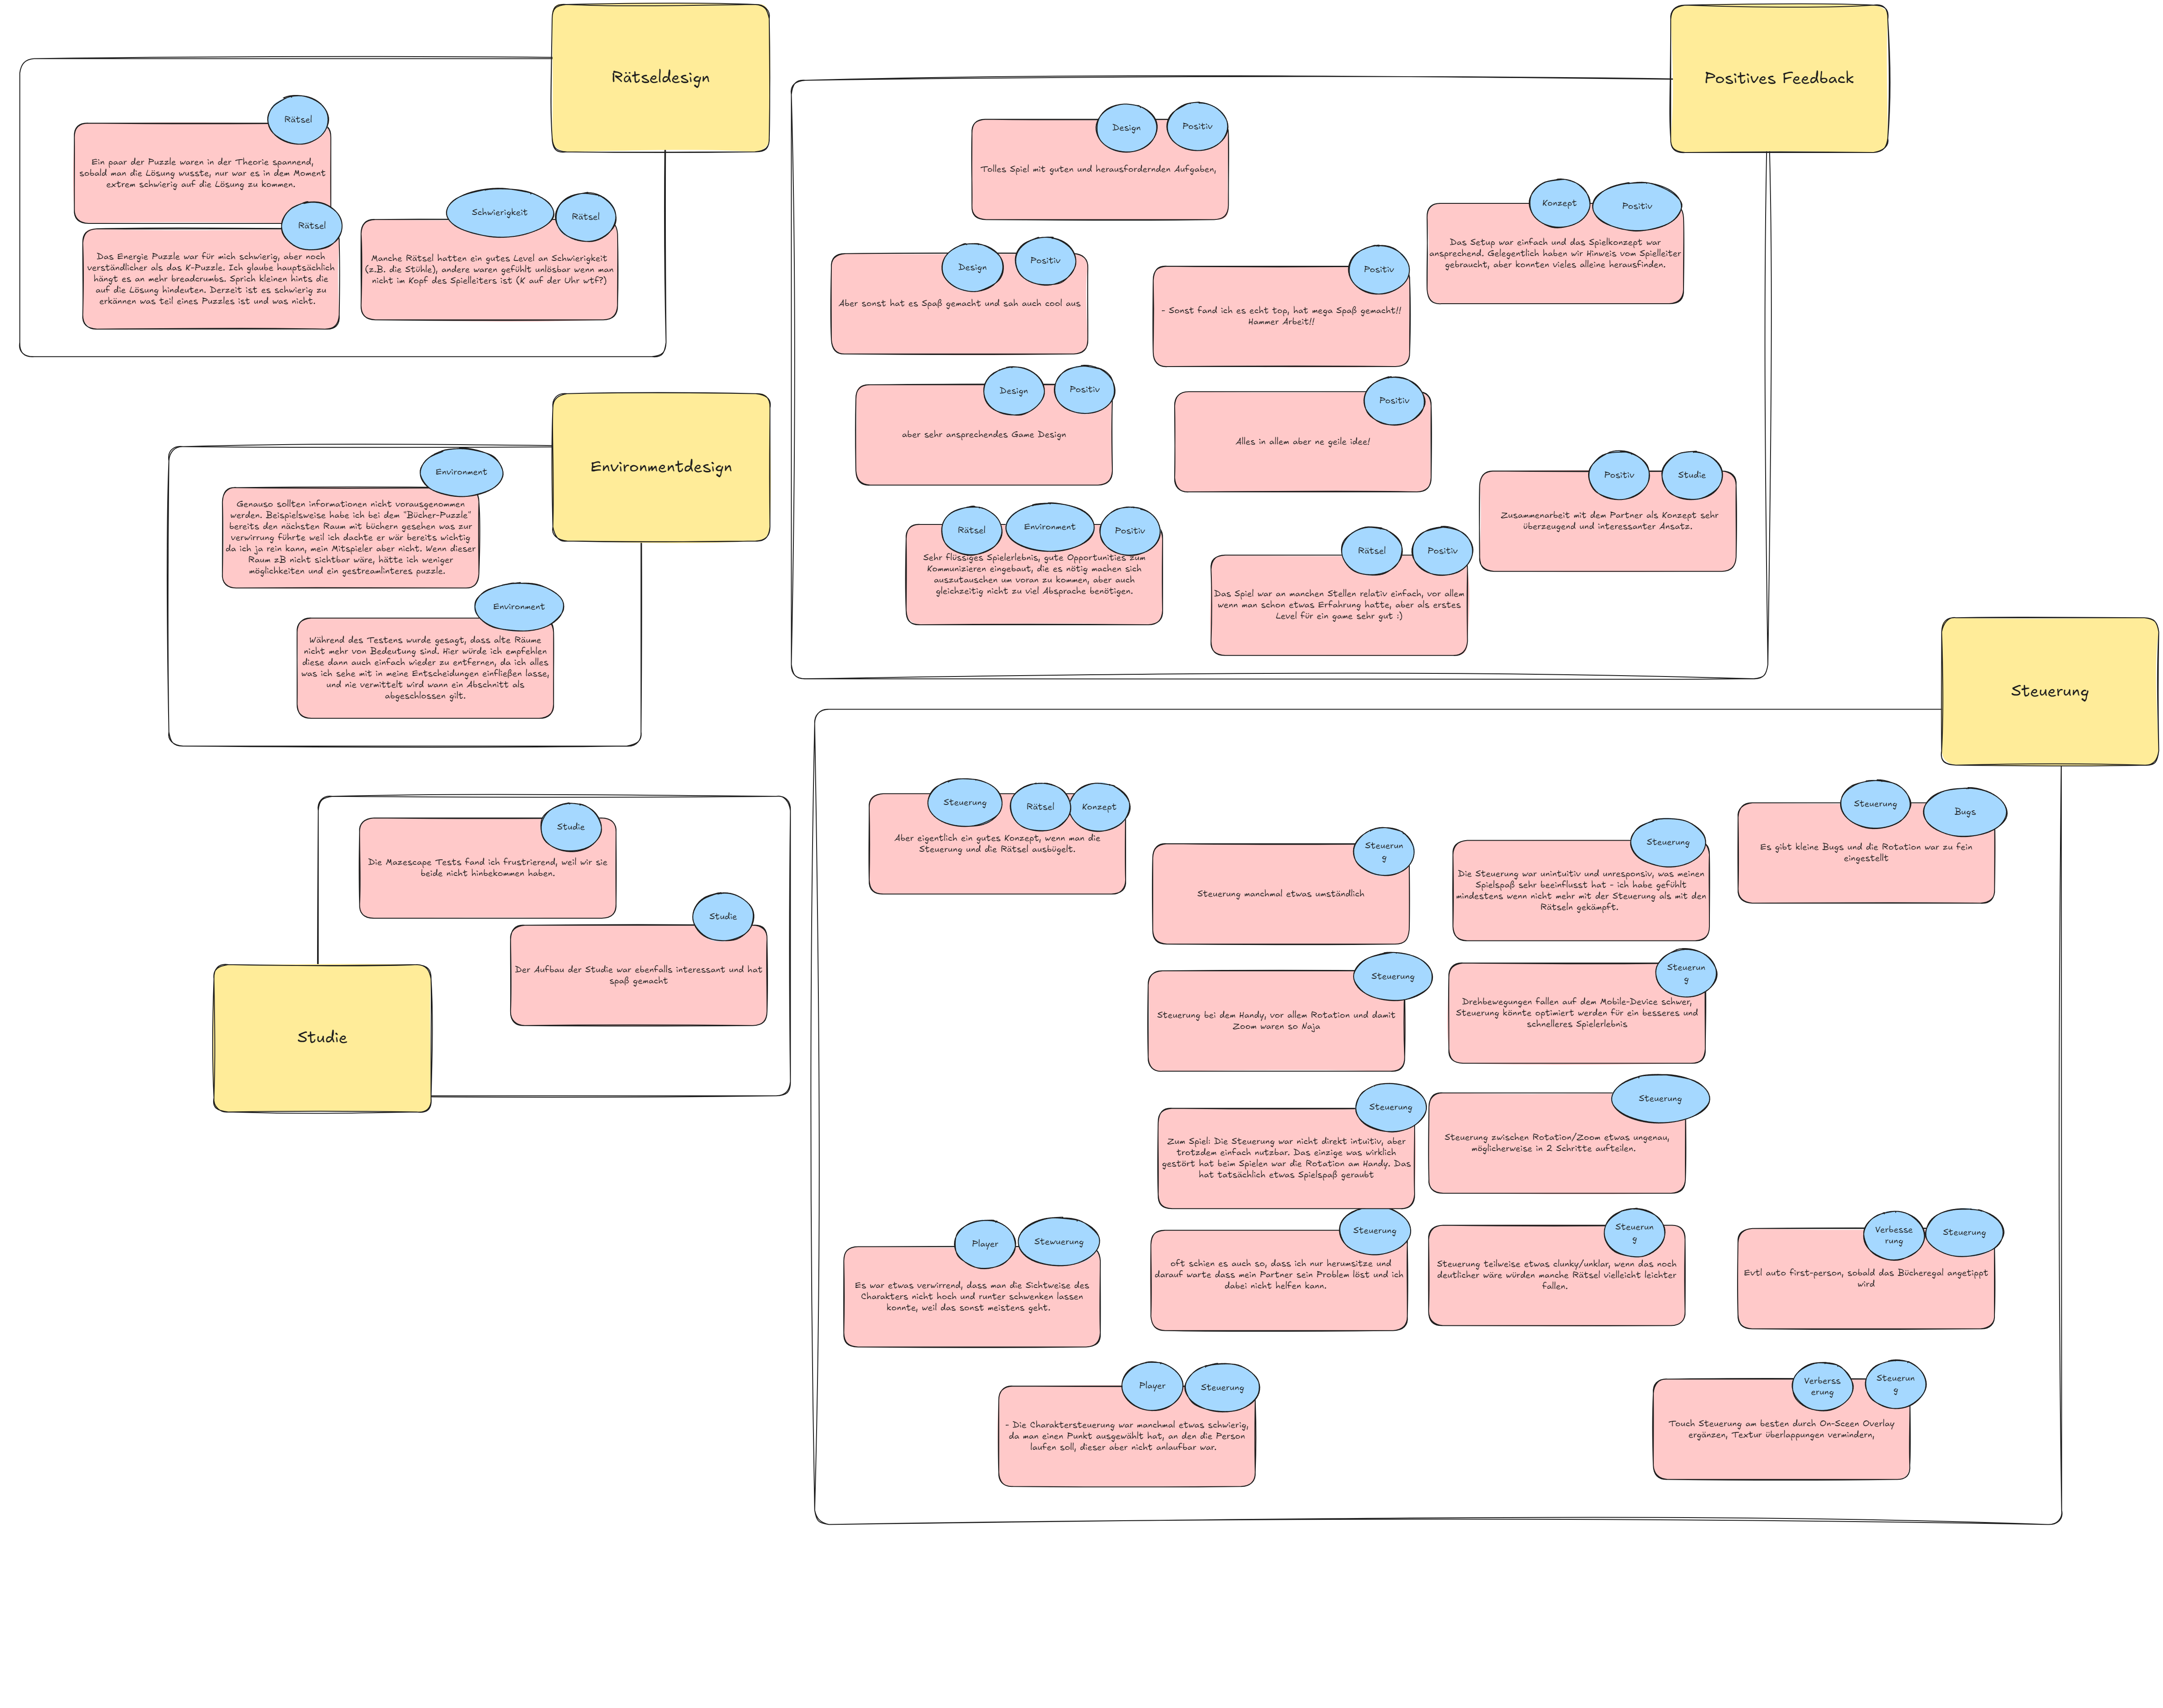
\includegraphics[width=1\linewidth]{content/pictures/Qualitative-Auswertung-Schritt-1.png}
\caption{Ergebnis der groben Kategorisierung nach \cite{braun_using_2006} (Quelle: eigene Darstellung)}
\label{fig:qualitative-results}
\end{figure}

Abbildung \ref{fig:qualitative-results-end} fasst die zentralen Rückmeldungen der Teilnehmer zusammen. Die Steuerung, insbesondere in der Watcher-Anwendung, wurde insgesamt als problematisch bewertet. Mehrere Kommentare beschrieben sie als umständlich, unintuitiv, träge (\say{unresponsiv}) oder \say{clunky} sowie als insgesamt unklar. Besonders betroffen waren dabei die Yaw- und Zoom-Gesten der \ac{3D}-Anwendung. Als mögliche Verbesserung wurde unter anderem die Integration unterstützender Elemente in das Overlay-\ac{UI} angeregt, um eine bessere Differenzierung zwischen der Zoom- und der Rotationsfunktion der Ansicht zu ermöglichen.

In der Player-Anwendung wurde das Fehlen einer vertikalen Kamerabewegung in der First-Person-Ansicht kritisiert, da derzeit nur eine fixe vertikale Perspektive genutzt werden kann. Zudem kam es mehrfach zu Schwierigkeiten bei der Auswahl einer Zielposition, zu der sich der Avatar bewegen sollte.

Hinsichtlich des Rätsel- und Umgebungsdesign wurde angemerkt, dass die Lösungsfindung teilweise noch unausgereift und zu herausfordernd sei. Es wurde vorgeschlagen, zusätzliche Hinweise in die Spielwelt zu integrieren, um die Rätsel zugänglicher zu gestalten. Weiterhin wurde empfohlen, bereits gelöste Räume zu deaktivieren, da diese andernfalls bei der Lösung neuer Aufgaben als irritierende Störfaktoren wahrgenommen werden. 

Die Nutzerstudie wurde insgesamt als interessant und professionell umgesetzt bewertet. Gleichwohl wurde der Vor- und Nachtest mit MazeScape vereinzelt als frustrierend empfunden.

Insgesamt wurde der Spielprototyp als unterhaltsam wahrgenommen. Das Spielkonzept von Connecting-Minds wurde als überzeugend und ansprechend umgesetzt bewertet. Positiv hervorgehoben wurde außerdem das einfache Setup.

\begin{figure}[ht]
\centering
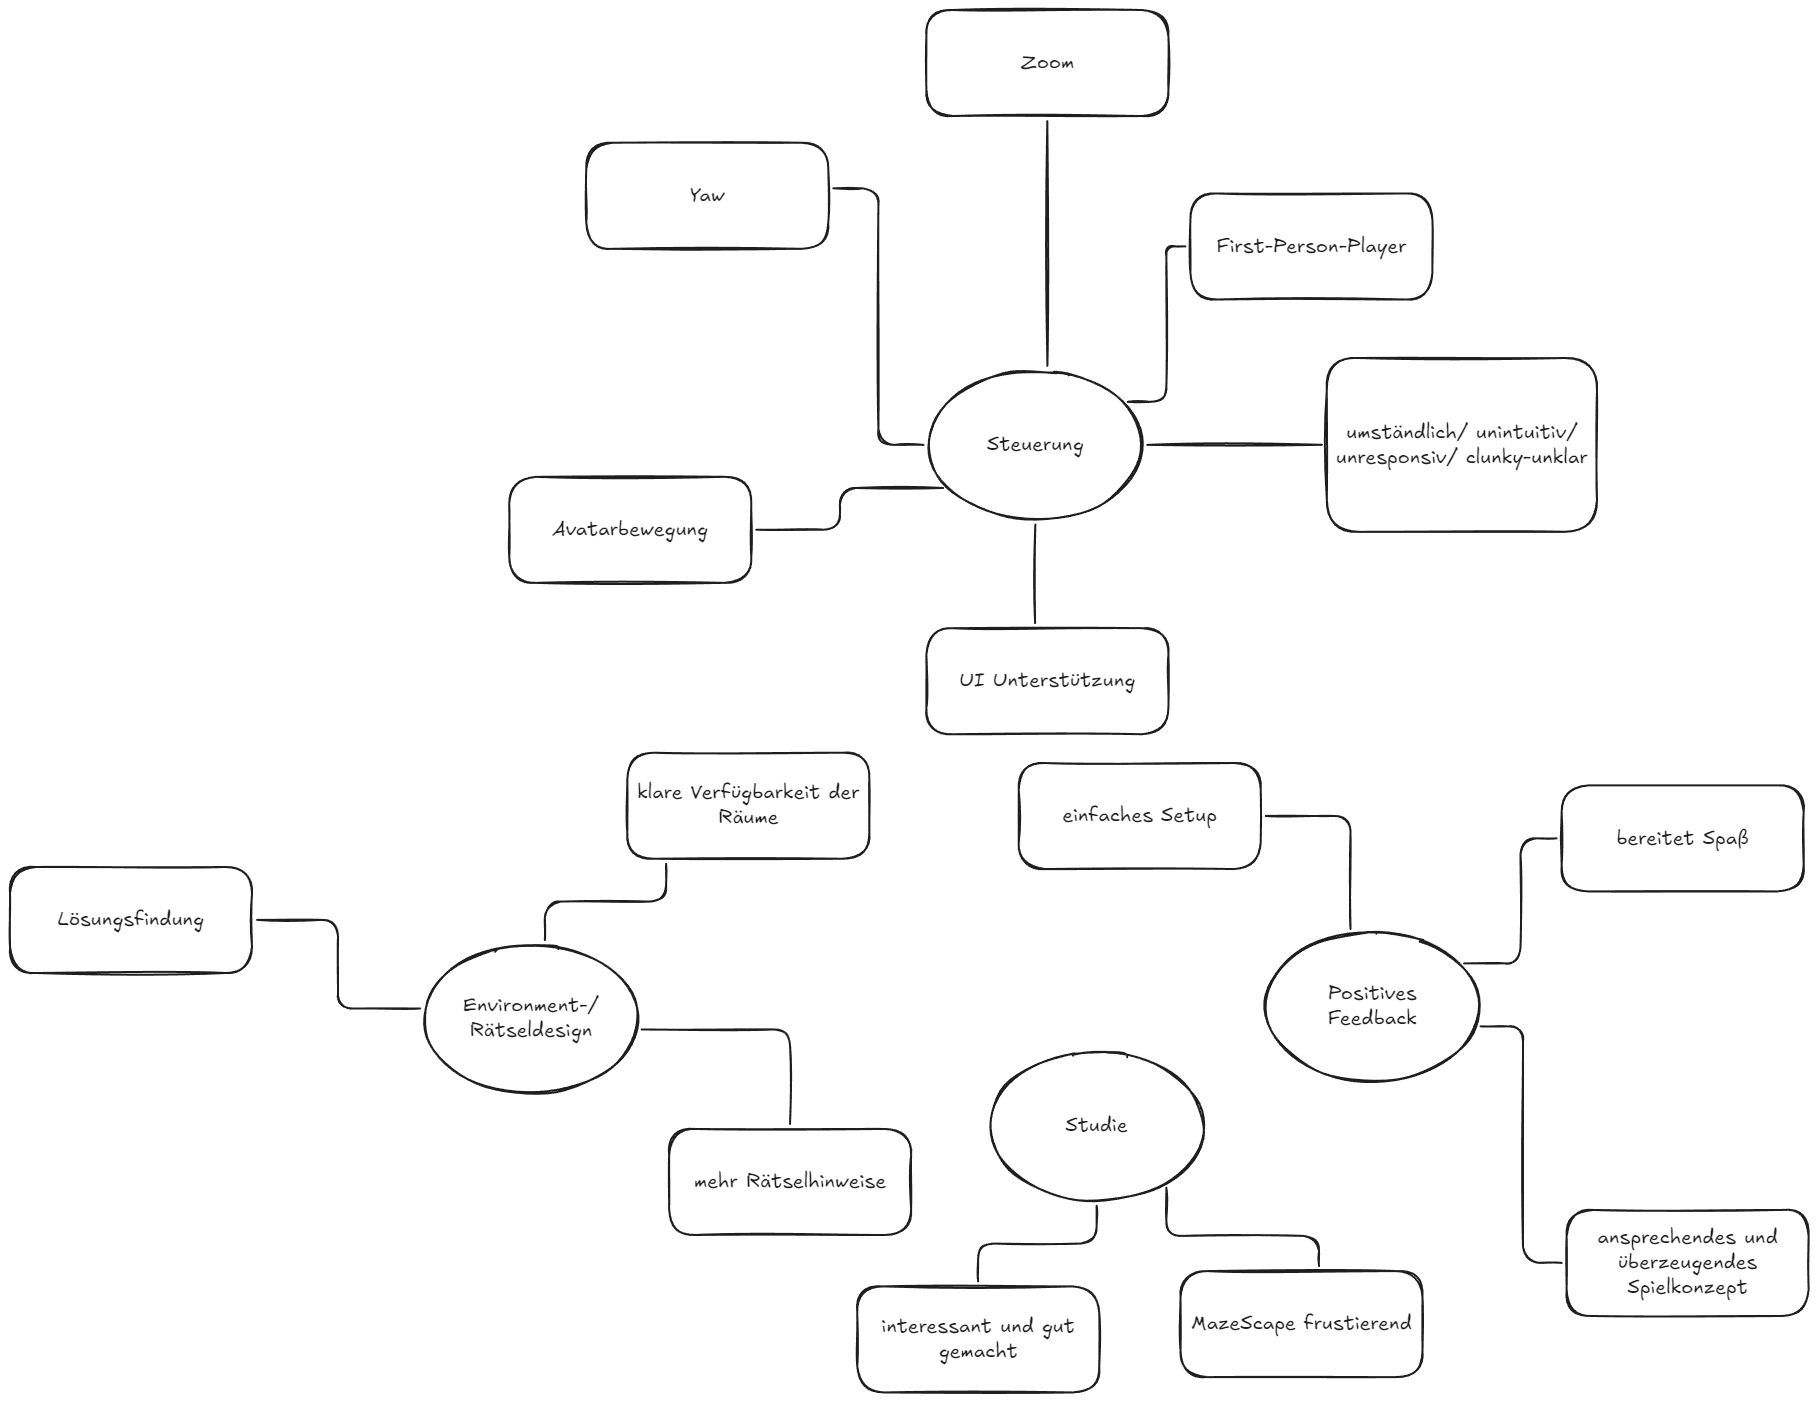
\includegraphics[width=1\linewidth]{content/pictures/Qualitative-Auswertung-Schritt-2.png}
\caption{Ergebnis der feinen Kategorisierung nach \cite{braun_using_2006} (Quelle: eigene Darstellung)}
\label{fig:qualitative-results-end}
\end{figure}

\subsection{Einordnung der qualitativen und quantitativen Ergebnisse}

Die Auswertung des Freitextfeldes liefert differenzierte Hinweise auf die Ursachen für den vergleichsweise niedrigen Wert im \ac{SUS}. Die eingeschränkte Gebrauchstauglichkeit lässt sich vor allem auf mangelnde Klarheit sowie auf die verbesserungswürdige Umsetzung der Steuerung in beiden Anwendungen, insbesondere jedoch in der Watcher-Anwendung, zurückführen. Darüber hinaus fließen auch die im Freitextfeld thematisierten Kritikpunkte am Rätsel- und Umgebungsdesign in die Bewertung ein.

Der durchschnittliche Frustrationswert im \ac{NASA-TLX} (M = 29,29) kann diese Einschätzungen nur teilweise stützen. Zwar liegt der Mittelwert im unteren Bereich, die hohe Standardabweichung von SD = 31 weist jedoch darauf hin, dass einzelne Teilnehmer ein deutlich höheres Maß an Frustration erlebten.

Demgegenüber zeigen die Ergebnisse des \ac{IMI} und des \ac{GEQ}, unterstützt durch das positive qualitative Feedback, dass die Probanden trotz der genannten Herausforderungen Interesse, Freude und Spielspaß entwickeln konnten.

\subsection{Vorstellung der gesammelten Auffälligkeiten bezüglich der konzipierten Rätsel}

In diesem Kapitel werden beobachteten Auffälligkeiten beschrieben, die während der Versuchsdurchführung festgestellt wurden, als die Probanden den Prototyp spielten. Die Beobachtungen beziehen sich insbesondere auf die konzipierten Rätsel und das Verhalten der Probanden im Umgang mit diesen. Es werden jene Rätsel thematisiert, bei denen es zu Problemen oder Schwierigkeit kam. Die dokumentierten Beobachtungen werden dabei in chronologischer Reihenfolge entlang des Spielverlaufs dargestellt.

Beim dritten Rätsel (vgl. Abbildung \ref{fig:riddle-design-section00-02}) hatten mehrere Probanden Schwierigkeiten, das intendierte Muster korrekt zu entschlüsseln. Dafür lassen sich mehrere Ursachen identifizieren. Zum einen lenkt das Passwort-Panel neben der Tür zu sehr von der eigentlichen Rätselumgebung ab, wodurch zunächst fälschlicherweise nach Passwörtern gesucht wurde. Zum anderen lasen einige Watcher die Beschreibung des relevanten Objekts nicht oder nicht sorgfältig genug, obwohl diese Hinweise zur Lösung enthielten. Erst nach einem gezielten Hinweise wurde die Lösung des Rätsels deutlich. Zusätzlich lenkten die verschlossenen Korridore im Eingangsbereich zum Sicherheitsraum ab, wodurch zunächst versucht wurde, diese weiteren Räume zu öffnen.

Auch das Rätsel um das Platzieren des Stromgenerators  (vgl. Abbildung \ref{fig:riddle-design-section01-01}) wurde wiederholt als herausfordernd wahrgenommen. Nachdem der Player mit dem Terminal interagiert hatte, wurde von den Watchern häufig nicht bemerkt, dass ein Außenbereich aktiviert worden war. Dieses Problem ist vermutlich auf unzureichende audiovisuelle Rückmeldungen im aktuellen Stand des Prototyps zurückzuführen. Der implementierte Benachrichtigungston wurde zudem von mehreren Probanden vermutlich nicht wahrgenommen.

Beim Stuhlplatzierungsrätsel im Konferenzraum (vgl. Abbildung \ref{fig:riddle-design-section02-02}) wurden zwei Hauptprobleme identifiziert. Zum einen ignorierten die Probanden teilweise intendierte Hinweise, zum anderen zeigte sich, dass die Entdeckungsmechanik noch nicht ausgereift genug ist. Um einen Gegenstand zu entdecken, muss der Player diesen aktiv durch Annäherung \say{freischalten}. Dies führte dazu, dass die Stühle nicht vollzählig entdeckt wurden, da nicht alle vom Player freigeschaltet wurden. Eine Verbesserung wäre hier, interaktive Objekte bereits beim Betreten des Raumes sichtbar zu machen, sodass der Watcher direkt einen vollständigen Überblick erhält. Zudem wurde das im Küchenraum platzierte Symbol für das richtige Stuhlmuster übersehen. Infolgedessen probierten die Probanden alle drei Stuhlmuster aus, bis sie das richtige gefunden hatten. Das nicht entdecken des Symbols in der Küche kann im Zusammenhang mit der geringen Gebrauchstauglichkeit der Watcher-Anwendung zusammenhängen, da die jeweiligen Nutzer Probleme beim Drehen der Ansicht hatten. Aus diesem Grund sahen sich die Probanden in der Küche nicht umfassend genug um.

Darüber hinaus stellte sich das Bücherrätsel in seiner aktuellen Ausgestaltung als zu einfach heraus, während die visuellen Hinweise in der Watcher-Anwendung zu unauffällig dargestellt wurden. In diesem Rätsel muss der Player zwei in der Spielwelt gefundene Bücher in das Bücherregal platzieren   (vgl. Abbildung \ref{fig:riddle-design-section02-03}). Auffällig war, dass die korrekte Lösung ohne strategisches Vorgehen nach maximal zwei Versuchen gelöst werden konnte. Dies deutet darauf hin, dass die Anzahl der möglichen Kombination zu gering war, sodass kein echter Suchprozess nötig war. Eine komplexere Rätselgestaltung mit mehreren Kombinationsmöglichkeiten hätte den Watcher stärker zur aktiven Hinweisrecherche angeregt. Zudem wurde das Bücherregal in der Watcher-Ansicht als visuell unzureichend gestaltet empfunden, was das genaue Erkennen der Bücherreihenfolge zusätzlich erschwerte. Der Player konnte das Rätsel ohne Hinweise des Watchers lösen.

\subsection{Vorstellung der Ergebnisse der subjektiven Wahrnehmung der Probanden}

Im Folgenden werden die Ergebnisse zur subjektiven Wahrnehmung der Probanden im Hinblick auf den \ac{IOS} sowie den \ac{SAM} dargestellt. Die Einschätzungen wurden zu zwei Messzeitpunkten erhoben. Einmal vor dem Vortest als \say{Ground Truth} und erneut nach dem Nachtest, um potenzielle Veränderungen im Erleben sozialer Nähe und affektiver Zustände im Verlauf des Experiments sichtbar zu machen.

\begin{figure}[ht]
\centering
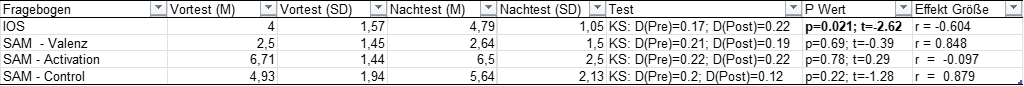
\includegraphics[width=1\linewidth]{content/pictures/IOS_SAM_Overal.png}
\caption{Ergebnisse des \ac{IOS} und \ac{SAM} auf alle Probanden bezogen (Quelle: eigene Darstellung)}
\label{fig:ios_sam_overal}
\end{figure}

Abbildung \ref{fig:ios_sam_overal} zeigt die aggregierten Ergebnisse der Erhebungen mittels \ac{IOS} und \ac{SAM}. Der analysierte Datensatz umfasst sowohl die Einschätzungen der Player- als auch die der Watcher. Eine differenzierte Betrachtung der Entwicklung innerhalb der einzelnen Rollen erfolgt im Anschluss in Abbildung \ref{fig:ios_sam_roles}.

Zur Vorbereitung der statistischen Auswertung wurde zunächst geprüft, ob die Daten eine Normalverteilung ausweisen. Für den Gesamtdatensatz erfolgt diese Überprüfung mittels Kolmogorov-Smirnov-Test. Die Teilstichproben wurden, analog zur Auswertung der Fragebögen zum Prototyp, zunächst visuell über \ac{Q-Q}-Plots begutachtet und anschließend mit dem Shapiro-Wilk-Test auf Normalverteilung getestet.

Lagen die Vor- und Nachtest-Daten normalverteilt vor, wurde ein t-Test für abhängige Stichproben durchgeführt, um mögliche signifikanten Veränderungen festzustellen. Zusätzlich wurde die Effektstärke berechnet. Für nicht-normalverteilte Daten wurde stattdessen der Wilcoxon-Test für abhängige Stichproben angewandt.

Zur Analyse der Differenzen zwischen den beiden Rollen wurde untersucht, welche Gruppe im Verlauf des Experiments stärkere Veränderungen aufwies. Für normalverteilte Subgruppen kam der Welch-Test zur Anwendung, bei nicht-normalverteilten Verteilungen wurde der Mann-Whitney-U-Test eingesetzt.

\paragraph{Allgemeine Auswertung}

Zunächst zeigt sich, dass die empfundene soziale Nähe innerhalb der Dyaden, gemessen über den \ac{IOS}, im Mittelwert signifikant ansteigt. Dieser Veränderung deutet darauf hin, dass sich die subjektive wahrgenommene soziale Nähe der Teilnehmenden im Verlauf des Experiments erhöht hat. Die zugehörige Effektstärke weist auf eine mittlere Korrelation hin.

Bezüglich der Valenz, also der affektiven Bewertung im Sinne positiver und negativer Emotionen (Bewertungsskala von 1 = \say{glücklich} bis 9 = \say{unglücklich}), zeigt sich im Mittelwert ein minimal Anstieg. Die Probanden konnten sich als ziemlich glücklich einschätzen. Die Veränderung ist jedoch statistisch nicht signifikant und weist lediglich eine sehr geringe Korrelation auf.

Auch die Erregung bzw. Aktivierung der Teilnehmer (Activation, Bewertungsskala von 1 = \say{aufgeregt} bis 9 = \say{entspannt}) steigt im Mittelwert leicht an. Insgesamt sind die Probanden zum Vortest und Nachtest recht entspannt aufgetreten. Die beobachtete Veränderung ist zu gering, als das sie signifikant sein kann. Außerdem weißt sie keine Korrelation auf.

Im Bereich der wahrgenommenen Dominanz (Control, Bewertungsskala von 1 = \say{fremdkontrolliert} bis 9 = \say{vollständig in Kontrolle}), zeigt sich ein höherer Anstieg des Mittelwerts als bei den zuvor gemessen Skalen. Sie zeigten eine ausgeglichene Dominanz. Auch diese Veränderung ist statistisch nicht signifikant und geht mit einer nur geringen Korrelation einher.

\paragraph{Auswertung in der Unterscheidung zwischen Player und Watcher}

\begin{figure}[ht]
\centering
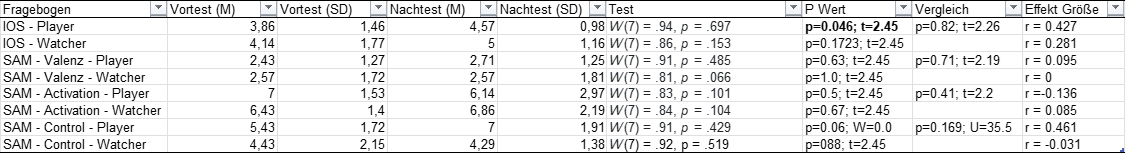
\includegraphics[width=1\linewidth]{content/pictures/IOS_SAM_Player_Watcher.png}
\caption{Ergebnisse des \ac{IOS} und \ac{SAM} auf beide Spielerrollen bezogen (Quelle: eigene Darstellung)}
\label{fig:ios_sam_roles}
\end{figure}

Der vollständige Datensatz wurde im Anschluss in die zwei Untergruppen Player und Watcher unterteilt und getrennt analysiert. Dabei zeigt sich, dass der signifikante Anstieg in der Entwicklung der sozialen Nähe ausschließlich bei den Teilnehmern der Player-Rolle festzustellen ist. In dieser Gruppe fällt auch die Korrelation höher aus als in der Watcher-Gruppe. Zwischen den beiden Gruppen konnte jedoch kein signifikanter Unterschied in der Veränderung der sozialen Nähe festgestellt werden.

In Übereinstimmung mit den Ergebnissen der Gesamtstichprobe zeigen sich auch in dem Subgruppen keine signifikanten Veränderungen in den Dimensionen Valenz, Activation und Control.

\subsection{Vorstellung der Ergebnisse der Quantisierung der Gesprächsflüsse}

In diesem Abschnitt werden die Ergebnisse der durchgeführten Vor- und Nachtests des Versuchsaufbaus dargestellt. Die Tests wurden jeweils pro Dyade aufgezeichnet und anschließend mithilfe von \say{whisperx} transkribiert (vgl. \citealp{bain_whisperx_2023}). Die Vorgehensweise zur Analyse der Transkripte orientierte sich an der Methode von \cite{nasir_effect_2015}, welche ein strukturiertes Verfahren zur quantitativen Auswertung vorgibt.

Zunächst wurden die Transkripte in einzelne Gesprächsblöcke unterteilt, die sich entweder durch längere Pausen oder durch einen thematischen Wechsel im Gesprächsverlauf voneinander abgrenzen ließen. Analog zur Definition bei \citeauthor{nasir_effect_2015} wurde eine Pause als ununterbrochener Zeitraum von mehr als drei Sekunden definiert, in dem keiner der Probanden spricht oder kommuniziert, ausgenommenen kurze Interaktionen.

Zur qualitativen Analyse des Gesprächsverlaufs wurden die Kommunikationsblöcke in sog.  \say{Floor Holding}-Muster unterteilt (vgl. \citealp{edelsky_whos_1981}). Floor Holding beschreibt dabei Situationen, in denen eine Person oder eine Gruppe von Personen den Gesprächsfluss für einen bestimmten Zeitraum dominiert (vgl. \citealp[S. 135]{nasir_effect_2015}). In Anlehnung darauf wird zwischen \say{\ac{CF}} und  \say{\ac{SF}} unterschieden. Während beim \ac{CF} beide Probanden aktiv am Gespräch teilnehmen und den Gesprächsverlauf gemeinsam gestalten, dominiert beim \ac{SF} nur eine Person das Gespräch, während die andere lediglich reagiert oder kurze Antworten gibt.

Darüber hinaus wurden die Gesprächsblöcke zeitlich codiert, um Beginn und Dauer innerhalb der Videoaufzeichnung präzise zu erfassen. So konnte bestimmt werden, wie lange die Gespräche jeweils andauerten und welchen relativen Anteil sie an der gemeinsamen Arbeitszeit des jeweiligen Tests einnahmen. Zusätzlich wurde, analog zur Methodik von \citeauthor{nasir_effect_2015}, die Anzahl der \say{Turns} gezählt, wobei ein Turn jeweils ein einzelner Redebeitrag eines Probanden darstellt. Ergänzend wurden auch die Wortzahlen pro Abschnitt erfasst, um diese später für Vergleiche zwischen den Teilnehmern und zwischen Vor- und Nachtest herziehen zu können.

Abschließend wurde die Gesamtzahl der gesprochenen Wörter pro Teilnehmer im jeweiligen Testdurchlauf erfasst. Diese wurde in Relation zur Gesamtwortanzahl des jeweiligen Tests gesetzt, um den individuellen Gesprächsanteil innerhalb der Dyade zu bestimmen.

Ergänzend zur Methodik von \citeauthor{nasir_effect_2015} wurde zusätzlich erhoben, welcher der beiden Probanden wie häufig Gesprächsblöcke initiierte. Dieser Indikator dient der Bewertung der Entwicklung kommunikativer Initiative im Verlauf des Experiments.

Zur statistischen Auswertung wurden die jeweiligen Stichproben zunächst mithilfe des Shapiro-Wilk-Tests auf Normalverteilung geprüft. Bei normalverteilten Stichproben wurden Veränderungen zwischen Vor- und Nachtest mittels t-Test für abhängige Stichproben ermittelt. Für den Vergleich unabhängiger Stichproben wurde der Welch-Test verwendet.

\begin{figure}[ht]
\centering
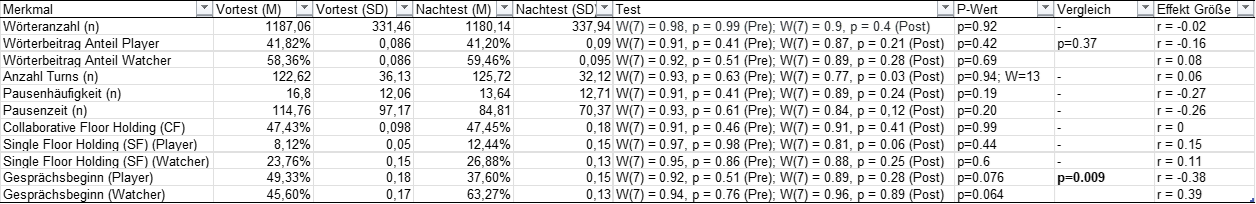
\includegraphics[width=1\linewidth]{content/pictures/quantitative_communication_results.png}
\caption{Ergebnisse des quantitativen Kommunikationsverhaltens aller Gruppen im Vergleich Vortest/Nachtest (Quelle: eigene Darstellung)}
\caption*{\footnotesize Das Kürzel (n) bezeichnet normalisierte Werte auf 10 Minuten Gesprächsdauer.}
\label{fig:communication-results}
\end{figure}

 Abbildung \ref{fig:communication-results} zeigt die Ergebnisse der quantitativen Analyse der einzelnen Probandendurchläufe. Abweichend von der Vorgehensweise von \citeauthor{nasir_effect_2015}, der eine testweise Auswertung vornimmt, wurde in dieser Untersuchung für jedes Merkmal der Mittelwert über alle sieben Testdurchläufe für Vor- und Nachtest berechnet.

 Die einzelnen Gruppen hatten jeweils 10 Minuten Zeit, um die kooperative Labyrinth-Aufgabe zu lösen. Einige Gruppen beendeten die Aufgabe vor Ablauf der Zeit, andere hingegen konnten sie innerhalb des vorgegebene Zeitrahmens nicht vollständig bearbeiten. Die durchschnittliche Bearbeitungszeit lag im Vortest bei M = 08:05 Minuten (SD = 02:27), im Nachtest bei M = 06:56 Minuten (SD = 03:15). Um Unterschiede in der Bearbeitungsdauer zu berücksichtigen, wurden die in Abbildung \ref{fig:communication-results} dargestellten Merkmale entsprechend normalisiert.

 Die durchschnittlich gesprochene Wortanzahl sank im Verlauf vom Vor- zum Nachtest leicht. Diese negative Veränderung erwies sich jedoch weder als signifikant noch als relevant im Hinblick auf die Effekt-Stärke. Zudem nahm die bereits im Vortest hohe Standardabweichung weiter zu, was auf eine größere Steuerung der Werte innerhalb der Gruppen hinweist.

 Die sprachlichen Beiträge der Probanden wurden jeweils anteilig zur Gesamtwortanzahl in ihrer Gruppe berechnet. Dabei zeigte sich ein leichter Rückgang der Wortanteile bei den Playern im Nachtest, während die Wortanteile der Watcher geringfügig anstiegen. Beide Veränderungen erwiesen sich jedoch weder als signifikant noch als substantiell korreliert. Die Anzahl der gemessenen Gesprächswechsel (Turns) stieg ebenfalls leicht an, allerdings ohne statistische Signifikanz.

Die Anzahl sowie die Dauer der Pausen innerhalb der Gesprächsprotokolle nahmen im Nachtest ab. Obwohl diese Veränderung statistisch nicht signifikant ist, deutet die mittlere negative Korrelation darauf hin, dass in längeren und häufigeren Szenarien eine signifikante Reduktion der Pausenzeiten möglich sein könnte. Eine Verringerung von Pausenanzahl und -dauer kann als Indikator für ein positives Kommunikationsverhalten gewertet werden.

Die Analyse des Floor-Holding-Verhaltens der Probandenpaare zeigt, dass das \ac{CF} im Mittelwert leicht zunahm. Bei den \ac{SF} der jeweiligen Teilnehmer war der Anstieg im Vergleich jedoch stärker ausgeprägt. Alle drei Veränderungen erwiesen sich als statistisch nicht signifikant. Auch die niedrigen Korrelationswerte lassen keine verlässliche Prognose zu, das in einem längeren Szenario mit größerer Stichprobe eine signifikante Verbesserung messbar wäre.

Die Auswertung der Gesprächsinitiativen ergab, dass die Probanden in der Player-Rolle im Nachtest seltener das Gespräch begannen als im Vortest. Umgekehrt zeigten die Watcher im Nachtest eine gesteigerte Initiative und eröffneten häufiger Gesprächssequenzen. Obwohl beide Veränderungen statistisch nicht signifikant sind, weisen sie eine mittlere Korrelation auf. Im Vergleich der beiden Untergruppen wurde jedoch ein signifikanter Unterschied festgestellt. Bei einer größeren Stichprobe könnten diese Entwicklung der Initiativen daher signifikant werden. Diese Entwicklung lässt sich auf die Funktionsart der Watcher-Anwendung herführen. Sie ist als koordinatives Glied gedacht und erwies sich dadurch in ihrer Wirkung als der primäre Initiierer der Gespräche.

Bezüglich der gemeinsamen Gesprächsführung konnten keine Verbesserungen festgestellt werden. Dennoch war eine Zunahme darin zu beobachten, dass die Anteile des \ac{SF} der Player und Watcher anstieg. Dies ist damit zu begründen, dass sie öfters versuchen die Probleme, vor denen sie im Nachtest standen, durch lautes denken zu lösen. Auch in diesem Bereich wurde keine signifikanten Unterschiede ermittelt.


\subsection{Vorstellung der Ergebnisse zum Thema Leadership}

In diesem Abschnitt werden die Ergebnisse des Leadership-Fragebogens nach \cite{emmerich_game_2016} im Zusammenhang mit den Resultaten der quantitativen Auswertung der Vor- und Nachtests dargestellt.

Zunächst wurde für jede Versuchsperson der Mittelwert der angegebenen Werte errechnet (Bewertungsskala von 1 = \say{trifft nicht zu } bis 5 = \say{trifft vollkommen zu}). Anschließend erfolgte die Berechnung des Gesamtdurchschnitts über alle Teilnehmer. Die Probanden zeigten insgesamt ein mittleres Maß an Führungskompetenz (M = 3.92; SD = 1.18). 

Zur Prüfung möglicher Unterschiede zwischen den Untergruppen Player und Watcher wurde zunächst mittel Shapiro-Wilk-Test die Normalverteilung der Daten überprüft. Der anschließende Vergleich der Mittelwerte erfolgt über einen ungepaarten t-Test.

Zwischen den Probanden der Watcher-Gruppe (M = 3.06; SD = 1.24) und der Player-Gruppe (M = 2.99; SD = 1.14) konnte kein signifikanter Unterschied festgestellt werden (p = 0.71; t = 2.18).

Abschließend wurde untersucht, ob ein Zusammenhang zwischen dem im Fragebogen gemessenen Leadership-Verhalten und der Anzahl der im Nachtest gesprochenen Wörter besteht. Zur Analyse dieser möglichen Beziehungen wurde der  Spearman'sche Rangkorrelationskoeffizient herangezogen.

\begin{figure}[ht]
\centering
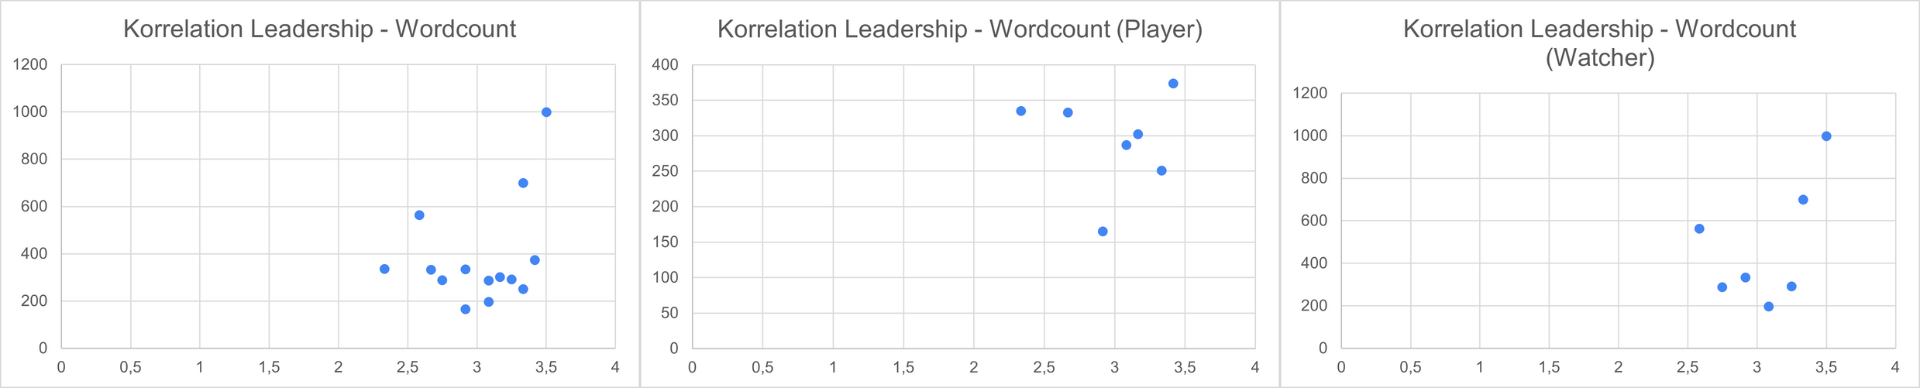
\includegraphics[width=1\linewidth]{content/pictures/Korrelation_Leadership_Wordcount_full.png}
\caption{Korrelation des Leaderships mit den gesprochenen Worten aus der quantitativen Gesprächsauswertung (Quelle: eigene Darstellung)}
\label{fig:correlation_leadership_wordcount}
\end{figure}

In Betrachtung aller Probanden in Bezug auf ihre durchschnittlichen Leadership-Werte zeigte sich lediglich eine sehr schwache Korrelation zur Anzahl der gesprochenen Wörter im Nachtest, die statistisch nicht signifikant war (rs(14) = 0.13; p = 0.66; (vgl. Abbildung \ref{fig:correlation_leadership_wordcount}, linkes Schaubild). Innerhalb der Untergruppe der Watcher konnte eine mittlere Korrelation festgestellt werden, die jedoch ebenfalls nicht signifikant war  (rs(7) = 0.46; p = 0.29; vgl. Abbildung \ref{fig:correlation_leadership_wordcount}, rechtes Schaubild). Für die Untergruppe der Player ergab sich keinerlei Korrelation (rs(7) = 0; p = 1; vgl. Abbildung \ref{fig:correlation_leadership_wordcount}, mittleres Schaubild).

Da in dieser Arbeit die Verbesserung der Kommunikation zwischen den Probanden im Vordergrund steht, liegt ein besonderer Fokus auf der Förderung kollaborativer Kommunikationsanteile. Wie bereits in der quantitativen Auswertung festgestellt wurde, zeigte sich keine signifikante Veränderung in den Anteilen des \ac{CF}. Die mittleren Werte der Leadership-Selbsteinschätzung deuten darauf hin, dass keiner der teilnehmenden Probanden eine dominante Führungsrolle einnahm. Dies könnte auf ein grundsätzlich kooperatives Kommunikationsverhalten hinweisen, bei dem Führungsaufgaben gleichmäßig verteilt und kooperative Kommunikationsformen bevorzugt werden.

Zur weiteren Analyse wurden die durchschnittlichen Leadership-Werte der Probanden berechnet, die gemeinsam an einem Testdurchlauf teilgenommen haben. Diese aggregierten Werte wurden anschließend mit den individuellen \ac{CF}-Anteilen innerhalb derselben Testdurchläufe verglichen.

\begin{figure}[ht]
\centering
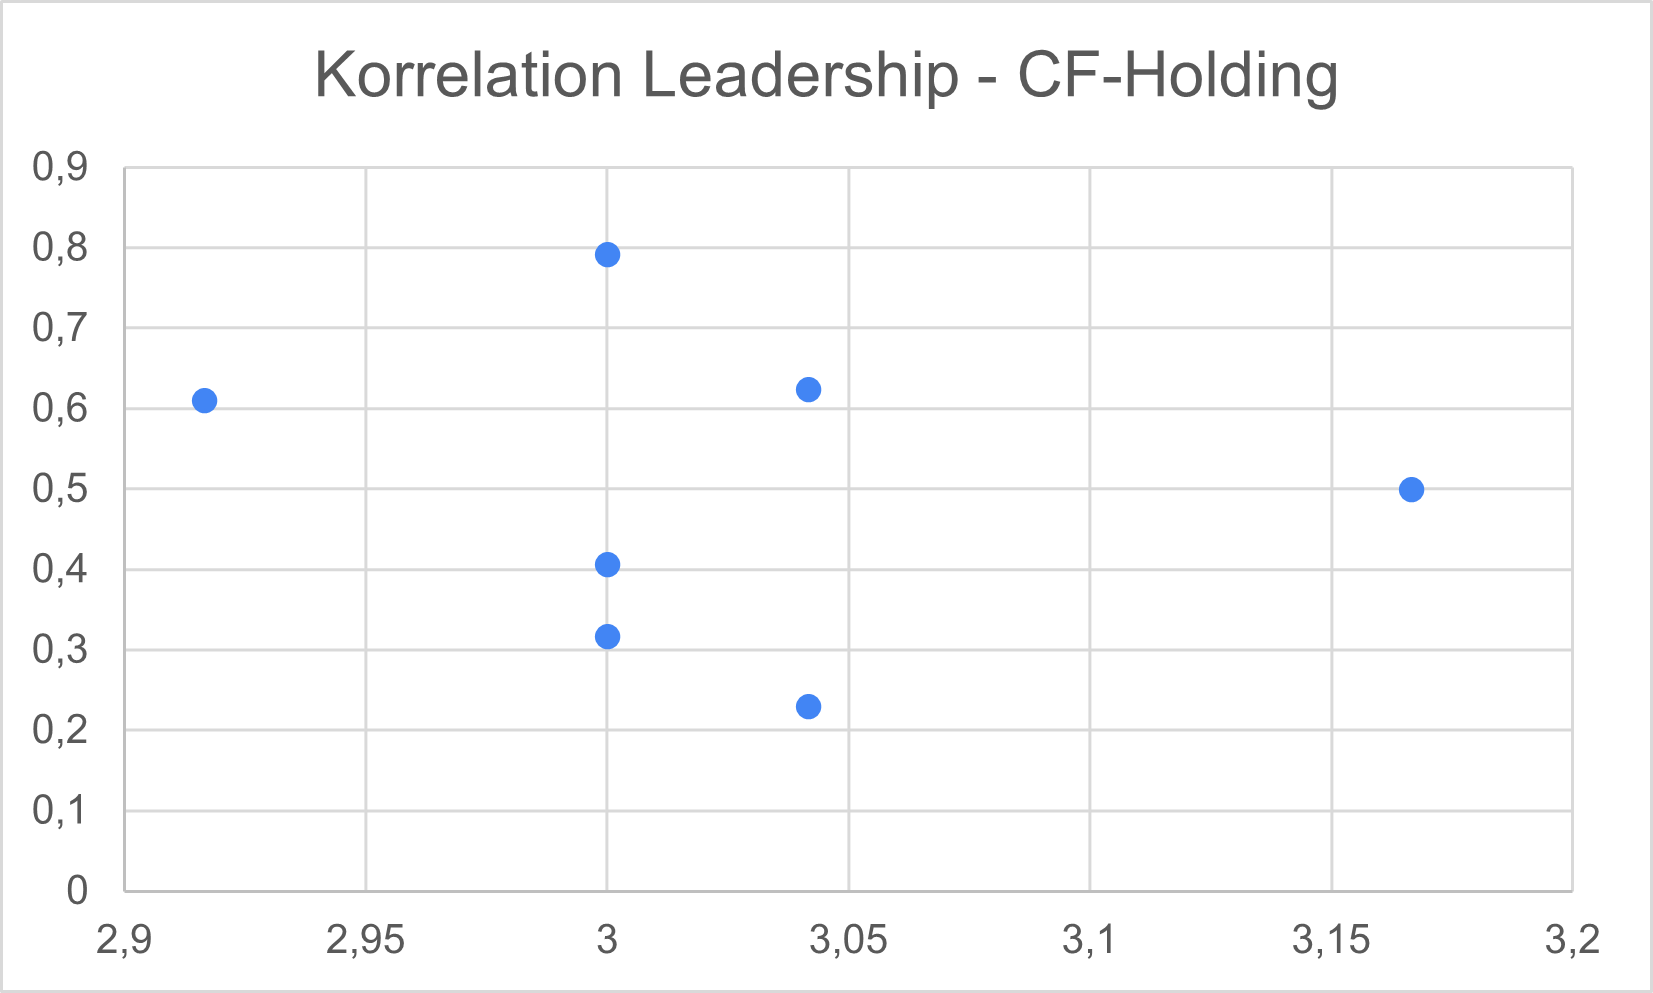
\includegraphics[width=1\linewidth]{content/pictures/korrelation_leadership_cfh.png}
\caption{Korrelation des Leaderships pro Probanden-Paar mit dem \ac{CF}-Anteil ihres Nachtests (Quelle: eigene Darstellung)}
\label{fig:correlation_leadership_cfh}
\end{figure}

Es konnte keine Korrelation  zwischen dem durchschnittlichen subjektiven Leadership-Empfinden der Dyaden und ihrem Anteil am \ac{CF} in den jeweiligen Nachtests festgestellt werden (vgl. Abbildung \ref{fig:correlation_leadership_cfh}). Diese Korrelation erwies sich zudem als statistisch nicht signifikant (rs(7) = -0.08; p = 0.86).

Im Anschluss wurde das subjektive Leadership-Empfinden mit den gemessenen Anteilen der Gesprächsinitiierungen verglichen (vgl. Abbildung \ref{fig:correlation_leadership_conversation_starts}). Weder in der Player-Gruppe  (rs(7) = -0.07; p = 0.88) noch in der Watcher-Gruppe (rs(7) = -0.03; p = 0.94) zeigten sich signifikante Korrelationen.

\begin{figure}[ht]
\centering
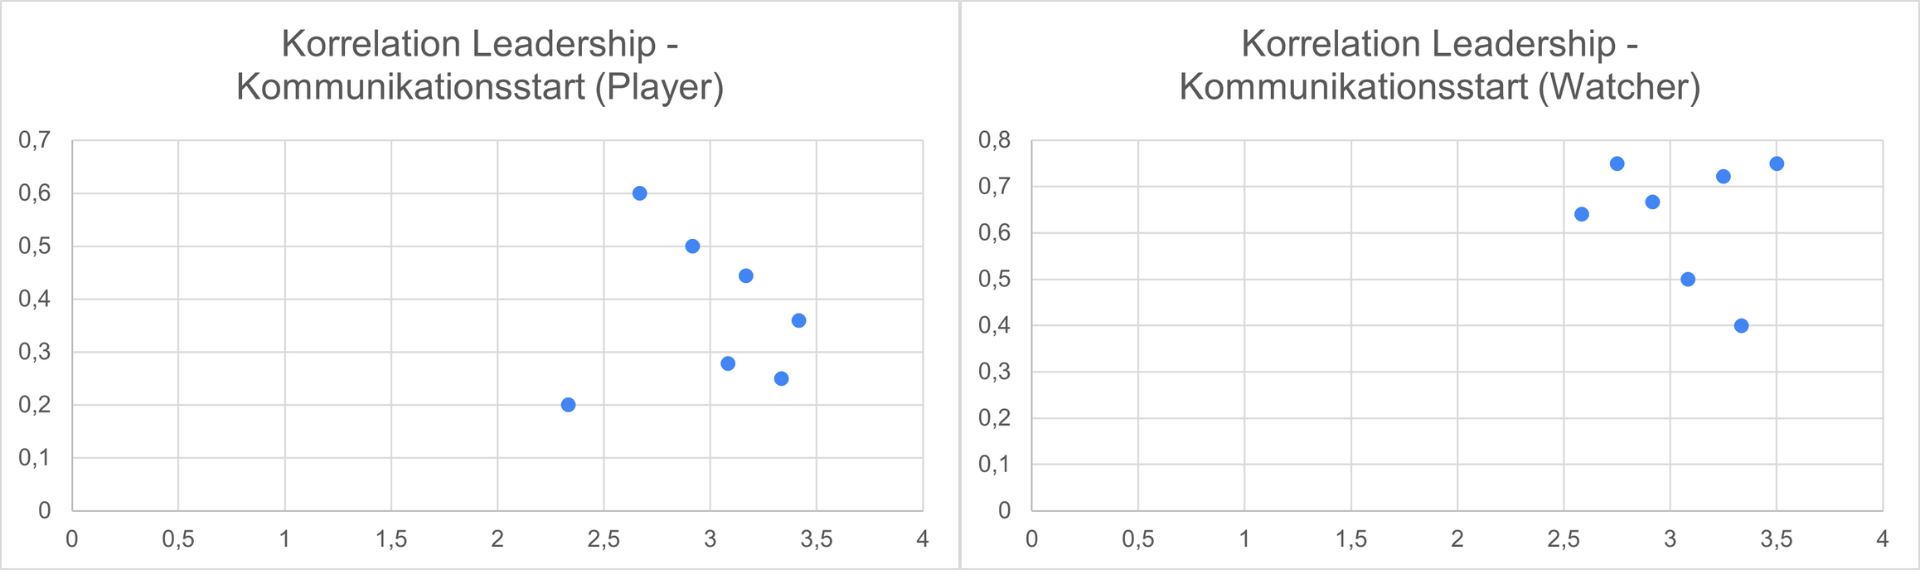
\includegraphics[width=1\linewidth]{content/pictures/Korrelation_Leaderhip_Start_of_conversation.png}
\caption{Korrelation des Leaderships von Player und Watchern mit dem Anteil der Konversationsstarts (Quelle: eigene Darstellung)}
\label{fig:correlation_leadership_conversation_starts}
\end{figure}

Insgesamt lässt sich festhalten, dass das durchschnittlich empfundene Leadership keine statistisch messbare Auswirkung auf die Kommunikationsentwicklung im Rahmen der quantitativen Untersuchung zeigt.

\subsection{Vorstellung der Ergebnisse zum Thema Kognitive Empathie}

In  diesem Unterkapitel werden die Ergebnisse des Fragebogens zur kognitiven und affektiven Empathie vorgestellt (Bewertungsskala von 1 = \say{Stimme überhaupt nicht zu} bis 5 = \say{Stimme voll und ganz zu}). Zur Erhebung der kognitiven Empathie wurden die Einzelwerte beider entsprechenden Subskalen addiert. Das Gesamtergebnis zeigt, dass die Probanden ein insgesamt hohes Maß an kognitiver Empathie ausweisen (M = 70; SD = 10.21; Maximalwert 95).

Ein ungepaarter t-Test bei ungleichen Varianzen ergab keinen signifikanten Unterschied zwischen den Subgruppen der Player (M = 68.71; SD = 9.96) und Watcher (M = 71.29; SD = 11.09), obwohl die Watcher im Mittelwert leicht erhöhte Ausprägungen aufwiesen.

\begin{figure}[ht]
\centering
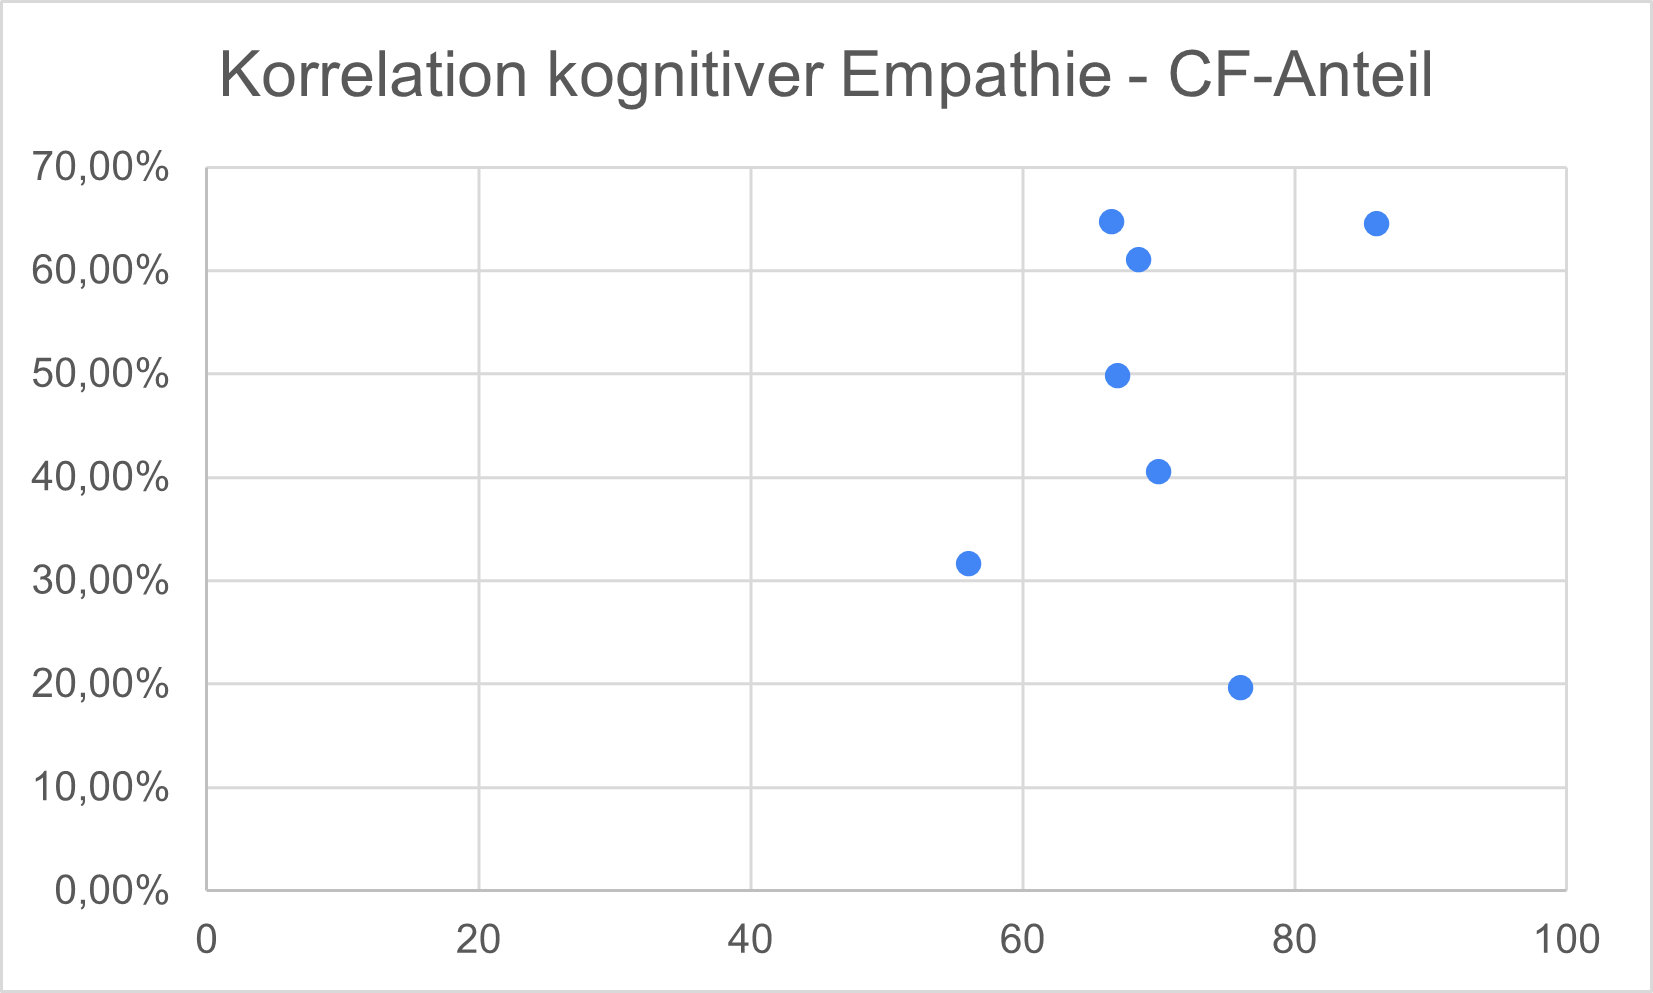
\includegraphics[width=1\linewidth]{content/pictures/Korrelation_Kognitive_Empathie_cfh.png}
\caption{Korrelation kognitiver Empathie mit \ac{CF}-Anteil pro Probanden-Paar (Quelle: eigene Darstellung)}
\label{fig:correlation_kognitive_empathy_cfh}
\end{figure}

Mittels Spearman´schem Rangkorrelationskoeffizienten wurde zudem geprüft, ob ein Zusammenhang zwischen dem Maß an kognitiver Empathie und dem Anteil am \ac{CF} im Nachtest besteht. Es konnte keine Korrelation festgestellt werden (rs(7) = -0.04; p = 0.94; vgl. Abbildung \ref{fig:correlation_kognitive_empathy_cfh}).

\subsection{Vorstellung der Ergebnisse zum Thema Fragen zum Nutzen eines spielerischen Ansatzes und Verbesserung der Kommunikation, insbesondere auch im Umgang mit nicht bekannten Personen}
\textbf{Anmerkung}: Nach Abschluss der Datenerhebung wurde festgestellt, dass die Fragebogenantworten eines Probanden nicht abgespeichert bzw. übermittelt wurde. Aus diesem Grund basieren die folgenden Auswertungen auf den Antworten von N = 13 Probanden.

Abschließend werden die Ergebnisse des letzten Fragebogens zum Thema \say{Fragen zum Nutzen eines spielerischen Ansatzes und Verbesserung der Kommunikation, insbesondere auch im Umgang mit nicht bekannten Personen} vorgestellt. Für diesen Themenbereich liegt bislang kein standardisierter Fragebogen vor. Der hier entwickelte Fragebogen (Bewertungsskala von 1 = \say{Stimme überhaupt nicht zu} bis 5 = \say{Stimme voll und ganz zu}) umfasst die folgenden Items:

\begin{enumerate}
    \item Spielerische Elemente erleichtern es mir, mit anderen Personen in Kontakt zu treten.
    \item Der Einsatz von Spielelementen (z. B. Aufgaben, Belohnungen, Avatare) kann die Kommunikation zwischen unbekannten Personen fördern.
    \item Ich bin offen dafür, neue Menschen kennenzulernen.
    \item Interaktive oder spielerische Funktionen in digitalen Anwendungen erleichtern mir den Austausch mit Anderen.
    \item Ich würde eine digitale Plattform nutzen, die durch spielerische Elemente den Kontakt zu mir unbekannten Personen erleichtert.
    \item Es fällt mir leichter, mit anderen Personen in Kontakt zu treten, wenn spielerische Komponenten involviert sind.
    \item Ich erkenne einen Mehrwert darin, spielerische Kommunikation in beruflichen oder sozialen Kontexten zu integrieren.
\end{enumerate}

Die Items 1, 2, 4 und 6 lassen sich der Kategorie \say{Gamification erleichtert soziale Interaktion} zuordnen. Item 5 bildet die Kategorie  \say{Akzeptanz / Nutzungsintention gamifizierter Plattformen}. Die Items 3 und 7 fassen die Kategorie \say{soziale Offenheit und Haltung zu spielerischer Kommunikation} zusammen.

Für die Auswertung der Fragebögen wurde analog zu den o. g. Fragebögen der Mittelwert pro Kategorie ermittelt.

Bezüglich der Kategorie \say{Gamification erleichtert soziale Interaktion} zeigt sich ein hoher Zustimmungswert unter den Probanden (M = 4.42: SD = 0.61). Zur \say{Akzeptanz / Nutzungsintention gamifizierter Plattformen} ergibt sich ein eher heterogenes Meinungsbild (M = 3.5; SD = 1.27). Hinsichtlich der \say{sozialen Offenheit und Haltung zu spielerischer Kommunikation} wurde eine tendenziell positive Einstellung deutlich (M = 3.77; SD = 0.95).

\section{Hypothesenüberprüfung}

Aufgrund des Umfangs des Forschungshintergrunds und des Versuchsaufbaus wurde die Anzahl der zu überprüfenden Hypothesen im Vorfeld der Nutzerstudie auf fünf begrenzt. Die im Vorfeld formulierten Thesen werden nun mit den empirisch erhobenen Ergebnissen aus der Nutzerstudie verglichen.

Die Auswertung der Fragebögen und Transkripte zeigt, dass mit Connecting-Minds ein Spiel entwickelt werden konnte, das durch seine Spielmechanik eine interessante und involvierende Erfahrung ermöglichte. Die intendierte Wirkung des Prototyps wurde jedoch durch Einschränkungen in der Gebrauchstauglichkeit der Steuerung gemindert, was sich negativ auf das Spielerlebnis auswirkte.

Dennoch konnte im Rahmen der Studie beobachtet werden, dass die soziale Nähe zwischen den teilnehmenden Personen gestärkt wurde, das auf eine grundsätzlich positive Wirkung des Prototyps hinweist. Aufgrund der geringen Stichprobengröße konnten jedoch keine statistisch signifikanten Veränderungen im Kommunikationsverhalten nachgewiesen werden, sodass eine empirische Bestätigung der zentralen Wirkannahme des Prototyps ausbleibt.

Nichtsdestotrotz legen die Ergebnisse nahe, dass die Anwendung dazu beitragen kann, Hemmschwellen im Erstkontakt mit unbekannten Personen zu reduzieren.

\begin{figure}[ht]
\centering
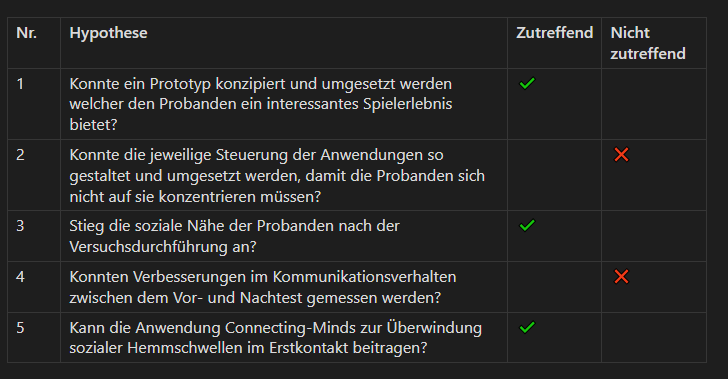
\includegraphics[width=1\linewidth]{content/pictures/Hypothesen_Nutzerstudie.PNG}
\caption{Hypothesenüberprüfung der Nutzerstudie (Quelle: eigene Darstellung)}
\label{fig:hypothesis_user_study}
\end{figure}

\section{Handlungsempfehlungen}

Auf Grundlage der Ergebnisse der quantitativen und qualitativen Datenerhebung wurden Handlungsempfehlungen abgeleitet und in ihrer Priorität anhand des Severity Rankings geordnet(vgl. Abbildung \ref{fig:call_to_actions_user_study}).

\begin{figure}[ht]
\centering
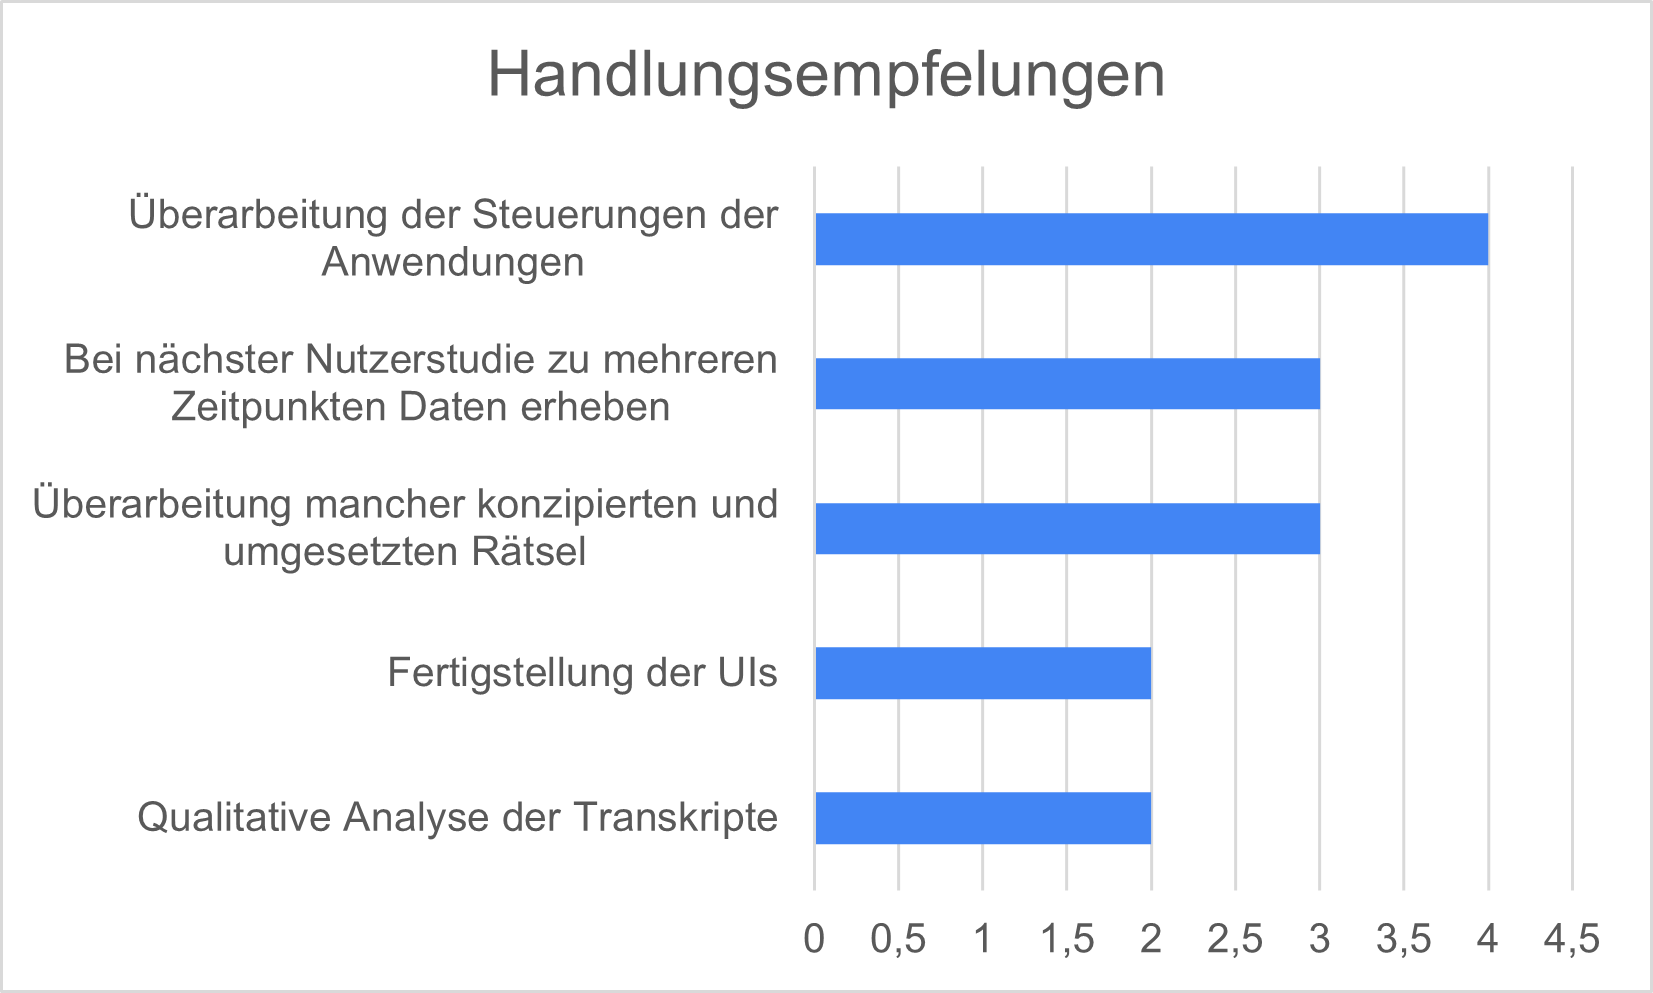
\includegraphics[width=1\linewidth]{content/pictures/Handlungsempfehlung_Nutzerstudie.png}
\caption{Handlungsempfehlungen zur Nutzerstudie (Quelle: eigene Darstellung)}
\label{fig:call_to_actions_user_study}
\end{figure}

Ein zentrales Augenmerk bei der Weiterentwicklung der Anwendungen sollte auf der Optimierung der Steuerung liegen. Nahezu alle Probanden kritisierten die Bedienbarkeit der Watcher-Anwendung, insbesondere im Hinblick auf die Unterscheidung zwischen der Yaw- und der Zoom-Geste. Eine klare Trennung oder feinere Differenzierung dieser Steuerungselemente wird von den Probanden explizit gewünscht.

Darüber hinaus zeigten sich konzeptionelle Schwächen einzelner Rätsel innerhalb des Prototyps. Diese erfordern weitere iterative Überarbeitungen. Für weiterführende Forschungsvorhaben in diesem Themenbereich ist zudem eine erweiterte Erhebungsstrategie zu empfehlen. So könnten etwa Instrumente wie der \ac{IOS} zu mehreren Messzeitpunkten, bspw. vor und nach dem Vortest, nach dem Prototyp, sowie nach dem Nachtest, eingesetzt werden. Gleiches gilt für Fragebögen zu den Themenbereichen Leadership und kognitiver Empathie.

Zusätzlich zur quantitative Analyse der Transkripte könnte eine qualitative Auswertung erfolgen, um Veränderungen im Kommunikationsverhalten zu identifizieren.

Abschließend ist festzuhalten, dass aufgrund des Umfangs des Projektes und der durchgeführten Studie nicht alle Elemente des Spiels vollständig konzipiert und umgesetzt werden konnten. So sind bspw. viele \ac{UI}-Elemente nur skizzenhaft ausgestaltet und bedürfen weiterer Ausarbeitung.

\section{Zusammenfassung und Interpretation der Ergebnisse}

Die Auswertung der Fragebögen zum Prototyp ergab, dass vor Durchführung einer großangelegten Nutzerstudie noch deutlich mehr Zwischentests mit freiwilligen Probanden notwendig gewesen wären, um frühzeitig auf Defizite in der Gebrauchstauglichkeit aufmerksam zu werden.

Trotz dieser Einschränkungen konnte durch die signifikante Zunahme der wahrgenommenen sozialen Nähe ein zentrales Ziel von Connecting-Minds erreicht werden. Das grundlegende Konzept lässt sich somit in die Kategorie jener Spiele einordnen, die das Potenzial besitzen, zwischenmenschliche Nähe zu fördern.

Um darüber hinaus signifikante Veränderungen in weiteren untersuchten Aspekten nachweisen zu können, sind weiterführende Studien mit einer größeren Anzahl an Probandenpaaren erforderlich. Die quantitative Analyse der Vor- und Nachtestdaten weist darauf hin, dass Veränderungen beim Gesprächsbeginn sowie eine Reduktion von Gesprächspausen nahe an der statistischen Signifikanz liegen. Aufgrund der geringen Stichprobengröße konnten diese Effekte jedoch nicht als signifikant gewertet werden. Die beobachteten Effektstärken deuten jedoch darauf hin, dass entsprechende Veränderungen bei einer größeren Stichprobe statistisch nachweisbar wären.

Trotz berechtigter Kritik hinsichtlich der Gebrauchstauglichkeit der Anwendungen konnte das Spielkonzept überzeugen. Die Rückmeldungen der Teilnehmer zeigt, dass der Prototyp Freude bereitete und Potenzial für eine Weiterentwicklung bietet. Zudem kann er dazu dienen, eine erste Hemmschwelle beim Kennenlernen fremder Personen zu nehmen.

\section{Methodendiskussion}

Die folgende Diskussion setzt sich kritisch mit dem geplanten und umgesetzten Versuchsaufbau sowie den eingesetzten Erhebungsinstrumenten auseinander. Dabei werden sowohl antizipierte als auch retrospektiv beobachtete Stärken und Schwächen aufgezeigt sowie Empfehlungen formuliert, wie diese in zukünftigen Studien gezielt verstärkt bzw. reduziert werden können.

Zunächst ist die Datenerhebung und Stichprobengröße zu betrachten. Durch gezielte Ansprache via E-Mail und Instant-Messaging-Dienste konnten 14 freiwillige Probanden rekrutiert werden. Diese Anzahl ist für die Fragebogenerhebung als grundsätzlich ausreichend einzustufen. Für die Gesamtanlage des Versuchs, insbesondere im Hinblick auf die Analyse der Kommunikationsprotokolle, stellt eine Stichprobe von sieben Dyaden jedoch eine klare Limitation dar. In der Folge konnten für bestimmte Merkmale der Kommunikationsquantität keine statistisch signifikanten Entwicklungen festgestellt werden . Für belastbare statistische Aussagen wäre eine Stichprobengröße von mindestens 28 Personen erforderlich gewesen (vgl. \citealp[S. 158]{cohen_power_1992}). 

Bezogen auf die Bewertung der Gebrauchstauglichkeit der Anwendung ist die Anzahl der Teilnehmer hingegen als adäquat zu bewerten. Nach  \citet[S. 3088]{karwowski_determining_2006} reicht eine geringe Anzahl von etwa sieben Testpersonen aus, um zentrale Probleme in der Gebrauchstauglichkeit identifizieren zu können.

Der finalen Konzeption der Versuchsaufbaus ging eine umfassende Literaturrecherche voraus, um festzustellen, welche Aspekte durch Fragebögen sinnvoll erfasst werden können. Im Anschluss wurde eine Auswahl jener Instrumente getroffen, die für den vorliegenden Prototyp bzw. das Studiendesign als besonders relevant eingeschätzt wurden. Dabei galt es auch, inhaltliche Redundanzen zwischen den Erhebungsinstrumenten zu vermeiden. Die Vielzahl von etwa 20 potenziell geeigneten Fragebögen erwies sich dabei als Herausforderung, da sie schnell zu Unübersichtlichkeit und redundanter Erhebung führen drohten. 

Im zweiten Schritt werden die Inhalte der eingesetzten Fragebögen kritisch reflektiert. Bei der Auswahl wurde versäumt, einen Fragebogen zur Erfassung der wahrgenommenen Interdependenz der Anwendungen zu integrieren. Ein solcher Fragebogen hätte Aufschluss darüber geben können, in welchem Maß die gegenseitige Abhängigkeit der beiden Rollen empfunden wurde. Die daraus gewonnenen Erkenntnisse hätten wertvolle Hinweise zur Überarbeitung der bestehenden Rätsel sowie zur Konzeption zukünftiger Aufgabe liefern können.

Zudem fehlte ein strukturierter Fragebogen zur Erhebung qualitativer Rückmeldungen. Die einzige Möglichkeit der Feedback bestand bislang in einer offenen Freitextfrage. Diese war jedoch zu unspezifisch formuliert (welches sonstige Feedback hast du?) und bot keine gezielte Strukturierung. Zielführender wäre gewesen, themenspezifische offene Fragen zu verwenden, die einzelne Aspekte der Nutzung des Prototyps gezielt adressieren, um differenzierte Rückmeldungen zu erhalten.

Im letzten Abschnitt werden methodische und technische Herausforderungen im Ablauf thematisiert. Der Versuchsaufbau erwies sich insgesamt als sehr komplex und umfasste zahlreiche Einzelschritte. So mussten die MazeScape-Labyrinthe in der korrekten Reihenfolge zusammengelegt werden, um sicherzustellen, dass die Probanden ihre Vor- und Nachtests in der vorgesehenen Abfolge absolvieren konnten. Auf technischer Ebene musste im Android-Build der Watcher-Anwendung die korrekte IP-Adresse des WebSocket-Server hinterlegt werden. Der Laptop, auf dem der Express-Server lief, durfte während der Tests nicht ausgeschaltet werden. Zudem war beim Player-Rechner sorgfältig auf das jeweils passende Netzwerkprofil zu achten. Nach der Unterzeichnung der Datenschutzerklärung war ein Internetzugang für die ersten Fragebögen erforderlich, anschließend musste jedoch vor Beginn des Prototyp-Tests auf das Netzwerk des TP-Link-Routers gewechselt werden, ohne dabei das Google-Formular versehentlich zu aktualisieren. Nach Abschluss des Spiels war ein erneuter Wechsel ins \ac{HFU}-Netzwerk notwendigen um die anschließenden Fragebögen auszufüllen. Diese umständlichen Netzwerkwechsel hätten durch den Einsatz eines  zusätzlichen Laptops vermieden werden können.

Die vergleichsweise lange Dauer der Versuchsdurchführung könnte potenziell weitere Teilnehmer abgeschreckt haben. Die gewählte Länge war jedoch aus inhaltlichen Gründen notwendig. Die Probanden sollten über einen längeren Zeitraum hinweg gemeinsam an einer Aufgabe arbeiten, um aussagekräftige Kommunikationsmuster erfassen zu können. Gleichzeitig durfte die Spielzeit des Prototyps nicht zu kurz bemessen sein, da dessen Wirkung erst  nach einer gewissen Dauer der Interaktion zur Entfaltung kommt. Erst durch wiederkehrende Handlungsmuster und Automatismen lassen sich die kommunikativen Potenziale der Anwendung erfassen.

Die Dauer der Tests wirkte sich auf die anschließende Transkription und Auswertung aus. Zur Unterstützung der Transkription wurde eine Software eingesetzt, die jedoch stark von der Tonqualität der Aufnahmen abhängig war. Da für die Aufzeichnungen lediglich eine geliehene Kamera zur Verfügung stand, war die Tonspur in mehreren Abschnitten unzureichend. Infolgedessen mussten große Teile der Transkripte manuell erstellt werden, ein Prozess, der etwa 14 Tage in Anspruch nahm. Für zukünftige Studien sollte dringend ein weiteres externes Mikrofon verwendet werden, um eine höhere Aufnahmequalität der verbalen Äußerungen sicherzustellen.

Im ursprünglichen Versuchsaufbau erfolgte die Anwendung durch die Teilnehmer über das im Seminarraum vorhandene Smartboard. Dabei zeigte sich, dass die Probanden häufig zu nah am Bildschirm standen und den verfügbaren visuellen Bereich daher nicht vollständig überblicken konnten. Aus diesem Grund wurde in der vorliegenden Untersuchung ein kompakter Touchmonitor (15 Zoll) eingesetzt, mit dem eine deutlich intuitivere Interaktion möglich war und der gleichzeitig den vollständigen Bildausschnitt abbildete.

Für die Auswertung der Kommunikationsprotokolle wurde ausschließlich der quantitative Ansatz nach \cite{nasir_effect_2015} herangezogen, da sich dieser aus informatikbezogener Perspektive als praktikabel erwies. Eine qualitative Analyse auf Grundlage der von \cite{baykal_collaboration_2023} entwickelten Taxonomie wurde hingegen nicht durchgeführt, da dieser weitere fundierte Kenntnisse voraussetzt, über die im Rahmen dieser Arbeit nicht verfügt wurde. Zudem müsste über diese Taxonomie hinausgegangen werden, um möglichst viele Aspekte, die in den Grundlagen Kapiteln zu den Kommunikationsmodellen vorgestellt wurden, abzudecken und zu analysieren. Diese Analyse würde zudem über den Rahmen dieser Arbeit gehen. Es ist jedoch anzunehmen, dass anhand der Taxonomie bereits erste Erkenntnisse zur Entwicklung der verbalen und paraverbalen Kommunikation der Probanden messbar gewesen wären.

Die Entscheidung, sich ausschließlich auf quantitative Methoden zu stützen, konnte bislang nicht vollständig validiert werden. Eine größere Stichprobe könnte in zukünftigen Untersuchungen dazu beitragen, belastbare Aussagen zu ermöglichen. Langfristig erscheint eine Kombination aus quantitativen und qualitativen Verfahren sowohl wünschenswert als auch methodisch angemessen.

Darüber hinaus wurden die zu Beginn definierten Spielerrollen in der Auswertung nicht berücksichtigt, da nicht alle vier Rollen durch die Probanden besetzt wurden. Es wäre aufschlussreich gewesen zu analysieren, inwiefern sich bestimmte Spielertypen, insbesondere Socializer, gegenüber anderen Rollen behaupten konnten. Allerdings wurde dieser Spielertyp im Rahmen der vorliegenden Studie nicht identifiziert.